

\documentclass[9pt,twocolumn,twoside]{pnas-new}
% Use the lineno option to display guide line numbers if required.

\articletype{CLASSIFICATION}%%%% Article topic/classification

\templatetype{pnasresearcharticle} % Choose template
% {pnasresearcharticle} = Template for a two-column research article
% {pnasmathematics} %= Template for a one-column mathematics article
% {pnasinvited} %= Template for a PNAS invited submission

\begin{document}


\title{Title}

% Use letters for affiliations, numbers to show equal authorship (if applicable) and to indicate the corresponding author
\author[a,c,1]{Author One}
\author[b,1,2]{Author Two}
\author[a]{Author Three}

\affil[a]{Affiliation One}
\affil[b]{Affiliation Two}
\affil[c]{Affiliation Three}

% Please give the surname of the lead author for the running footer
\leadauthor{Lead author last name}

% Please add a significance statement to explain the relevance of your work
\significancestatement{Authors must submit a significance statement between 50 and 120 words in length about the significance of their research paper written at a level understandable to an undergraduate educated scientist outside their field of speciality. The primary goal of the significance statement is to explain the relevance of the work in broad context to a broad readership. If submitting a Direct Submission, please add a significance statement to explain the relevance of your work. Brief Reports do not publish with a significance statement, and should be omitted for this article type.}

% Please include corresponding author, author contribution and author declaration information
\authorcontributions{Please provide details of author contributions here.}
\authordeclaration{Please declare any competing interests here.}
\equalauthors{\textsuperscript{1}A.O.(Author One) contributed equally to this work with A.T. (Author Two) (remove if not applicable).}
\correspondingauthor{\textsuperscript{2}To whom correspondence should be addressed. E-mail: author.two\@email.com}

% At least three keywords are required at submission. Please provide three to five keywords, separated by the pipe symbol.
\keywords{Keyword 1 $|$ Keyword 2 $|$ Keyword 3 $|$ ...}

\begin{abstract}
    Abstract

    % \lipsum[1-2]
% Social interactions can shape how genetic variation is expressed and exposed to selection, potentially linking short-term ecological responses with longer-term evolutionary change. We extend models of indirect genetic effects by incorporating an explicit polygenic genetic architecture into an individual-based simulation of quantitative trait evolution, comparing three mechanisms by which social groups affect individuals: copying the group average, the fittest group member, or the most extreme group member. Under stabilizing selection, these mechanisms produced distinct genotype–phenotype relationships, and stronger social influence generally increased genetic variation, suggesting that social effects can relax the exposure of genetic variation to selection. A rare-mutant invasion analysis showed this same relaxation favors the spread of social behavior itself: copying the average or the fittest group member could always invade an asocial population, while copying the most extreme member invaded only below a threshold interaction strength set by group size. After an environmental shift, only copying the fittest group member produced an immediate adaptive phenotypic response, but this short-term benefit came at the cost of slower long-term genetic adaptation; in fluctuating environments, the fitness consequences of sociality instead depended on the interaction rule, shift magnitude, and fluctuation frequency. Together, these results show that whether sociality helps or hinders adaptation depends on what individuals copy, how strongly they copy, and how the environment changes.
\end{abstract}

\dates{This manuscript was compiled on \today}
\doi{\url{www.pnas.org/cgi/doi/10.1073/pnas.XXXXXXXXXX}}


\maketitle
\thispagestyle{firststyle}
\ifthenelse{\boolean{shortarticle}}{\ifthenelse{\boolean{singlecolumn}}{\abscontentformatted}{\abscontent}}{}

\Firstpage

% \section*{Introduction}

Many quantitative genetic models built on the classical Darwinian paradigm assume a direct genotype-phenotype mapping, in which an individual's phenotype is determined by its own genotype and a generic, non-social environment~\cite{Falconer1996}. However, this assumption is challenged once social interactions are taken into account, because part of the envrionment is made up of the genotypes and phenotypes of interacting conspecifics~\cite{Moore1997, Mousseau2009}. When organisms interact with each other, certain phenotype may be affected depending on who the interacting partner is and what the nature of the interaction is. For example, . Such a phenotype is termed a social interacting phenotype, a trait whose expression is affected by interactions with conspecifics \cite{Moore1997}.

In order to understand the evolutionary consequences of such social interacting phenotype, Moore et al. proposed a quantitative genetic model that partitioned the phenotype into a direct genetic contribution from one's own genotype, and an indirect genetic contribution from a social partner genotype~\cite{Moore1997}. They predicted that the evolutionary response of a social \Parasplit interacting phenotype should differ, often be greater, compared to a nonsocial phenotype, especially when the same trait in affected between social partners reciprocally, creating a feedback loop that drives phenotype evolution. Many extensions of this model have since been developped within the quantitative genetic framework~\cite{Wolf1999, McGlothlin2010, Bijma2008, agrawal2001, Bailey2014, Bailey2012} and simulation~\cite{Montiglio2017}. Empirical studies has estimated the value of the proposed interaction coefficient, $\psi$, in empirical systems~\cite{Bailey2017, Bijma2013}. Despite its theoretical importance as a central parameter to indirect genetic effect models, it is more difficult to measure $\psi$ than using other approaches such as variance partitioning, to meansure the effect of social partners' genotype on one's phenotype~\cite{Bailey2021}. 

Despite its influence, Moore et al.'s framework leaves two aspects of social interaction trait evolution underspecified. First, the model does not formalize who a focal individual interacts with or how that structure is determined; when extended to larger group size, many model assumed the average of all individuals in the group is influencing the focal individual \cite{McGlothlin2010}. This gap can be filled with evolutionary social learning theory which provides a formal definition for who, when and what individuals copy, known as social learning strategies \cite{Rogers1988,Laland2004,Rendell2010}. Second, Moore et al.'s quantitative genetic framework does not specify an explicit genetic architecture linking genotype to the interacting phenotype. Such omission misses the connection to a large body of empirical studies which infer selection on social interacting phenotype from molecular signature like dN/dS~\cite{Viljakainen2009, Roux2014, Harpur2013, Hunt2011, Warner2019}. In order to make the comparison, explicit mapping between genotype and phenotype is required in the modeling to generate falsifiable predictions about the evolutionary path of an interacting trait.

In this study, we built an population genetic individual-based model with explicit genetic architecture to test how social learning strategies -- copy-the-average, copy-the-best, or copy-the-extreme -- affects the evolution of a socially interacting trait. For each strategy, we varied the strength of social interaction and compared social and asocial populations under three selection regimes: stabilizing, directional, and fluctuating selection. In addition, we used an invasion analysis to test whether each strategy can invade an asocial resident population, a prerequisite for a fully social population to arise in the first place. We found that whether sociality helps or hinders adaptation depends on the interaction strategy, strength of interaction, and the stability of the envrionment.





% However, the field of population genetics argues that sociality in general should relax selection instead of intensifying it. The theory assumes that social structure segments a population into breeding groups characterized by reproductive skew, in which few individuals contribute to the offspring population~\cite{Linksvayer2009}. Group formation leads to both higher inbreeding than a well-mixed population, and fewer breeding individuals. Both structural changes lead to stronger drift and less effective selection at genome-wide level~\cite{Linksvayer2009, Romiguier2014}. It has been shown in spiders and ants that there is genome-wide elevated molecular evolution in social species compared to nonsocial relatives, suggesting relaxed selection~\cite{Tong2022, Agnarsson2012, Settepani2016, Mattila2012, Bechsgaard2019, Kapheim2015}. 

% Such debate between relaxed selection or accelerated adaptation also exist in empirical work. As a general example, immune genes are expected to be under different selection for social living species relative to solitary ones. Social interactions, especially group living, increases contact rate and relatedness among individuals, providing the ideal condition for disease transmission~\cite{SchmidHempel1998, Cremer2007}. Immune health depends on both genotype and environmental condition such as pathogen exposure in early life, and social interactions such as grooming and hygenic behaviors~\cite{Georgiev2016, Bulmer2021}. In ants and honeybees, it has been shown that immune genes have elevated dN/dS relative to Drosophila immune genes or non-immune genes in bees, which can be a signiture of either relaxed or positive selection~\cite{Viljakainen2009}. Studies have shown support for both sidess: enrichment of immunity genes for positive selection was shown in~\cite{Roux2014}, while~\cite{Harpur2013} provided support for relaxed purifying selection. Within the same broad functional category and same selective pressure cause from social living, there is no convergent agreement on whether the dominant signiture is relaxed constraint or adaptive acceleration, and the conclusion is gene-, taxon-, and method-dependent~\cite{Otani2016, Viljakainen2015}.

% While immune genes show both positive and relaxed selection in parallel, another gene family shows a different selective pattern when it is affected by the highest level of sociality. Eusocial speices evolved division of labor where members of the colony is divided into different castes with specific tasks such as foraging or nursing. Besides genetics, an individual's caste in adulthood also depends on the social interactions: diet received in larval stage, chemical signals released by other members, and age or immediate need of the colony~\cite{Schwander2010}. These are important factors for an individual to develop or switch to a specific caste. Given different social groups, genes that are caste-biased are expressed differentially and has shown elevated rate of evolution compared to noncaste-biased genes, similar to that of immune genes~\cite{Hunt2011}. Unlike immune genes, the evidence suggested that the caste-biased genes may undergo relaxed constraint followed by caste-specific positive selection~\cite{Hunt2011, Roux2014}. Most of the caste-associated genes are lineage-dependent and evolutionarily younger, suggesting caste-specific positive selection following the evolution of eusociality and division of labor~\cite{Warner2019}. Rather than both modes of selection happening in parallel, these socially influenced genes in eusocial species suggest that both modes can happen sequentially, adding complexity beyong what previous theory predicted. 

% Across theoretical and empirical studies, the same pattern emerges where a socially influenced trait evolves faster or slower is not predicted by whether a species is social, but by the specific structure of the interaction. Another field that similarly stresses the structure of social interactions is social learning theory. Rogers' paradox is a fundational result in this literature, stating that unconditional social learning does not raise mean population fitness; instead, the fitness payoff depends on who, when, and what individuals copy, formalized as social learning strategies~\cite{Rogers1988, Laland2004, Rendell2010}. Social learning strategies further decompose social group by specifying who is copied, offering a more fine-grained perspective than the coarser sociality measures used in the theories discussed above. In this study, we incorporate social learning strategies and explicit genetic architecture into a social interaction model extended from Moore et al.~\cite{Moore1997}. Given the complex, structure-dependent selection patterns observed in empirical systems, we test social populations under different selection modes in an attempt to characterize how different social learning strategies shape population-level evolutionary outcomes. 
 

\bibliography{pnas-sample}

\end{document}



\section*{Model}
Here we describe the overall structure of our model before detailing the three social interaction rules (\ref{sec:interaction_models}), the three selection regimes (\ref{sec:selection_regimes}), invasion analysis on whether sociality can establish itself (\ref{sec:invasion_analysis}), and simulation implementation (\ref{sec:simulation_details}) (these parentheses should point to subsections). Our model builds on two existing frameworks: the IGE model proposed by \cite{Moore1997} and the evolutionary quantitative-genetic framework developed by~\cite{Hayward2022}. \citep{Moore1997} specifies how social partners' genotypes enter the phenotype but leaves the genetic architecture of the trait unspecified, while \citep{Hayward2022} provide an explicit polygenic architecture under stabilizing and directional selection without modeling social interactions. In our model combined from these two models, an individual's phenotype is affected both by its own highly polygenic genotype and by its social partners. The genotype of the trait under selection follows the standard additive model with a highly polygenic genetic basis \cite{Hayward2022, Falconer1996}. One individual's genotype is given by

\begin{equation}
g = \sum_k a_{k},
\label{g_def}
\end{equation}
where $a_k$ is the effect size of the $k^{th}$ mutation carried by the individual.

The social interaction model is inspired by \cite{Moore1997}; we extend it to allow groups of more than two social partners as well as nonlinear interaction rules. In each generation, individuals are randomly partitioned into groups of $n$ individuals ($n\geq 2$), and group members act as each other's social partners for that generation. An individual's phenotype is then defined as
\begin{equation}
\label{eq:z_def}
z = (1-\psi)g+\psi g_{social} +e,
\end{equation}
where $\psi$ is the interaction coefficient, $g_{social}$ is the indirect genetic effect contributed by the individual's social partners, and $e$ is a general environmental effect. $\psi$ is held constant within a simulation; $g_{social}$ is calculated differently depending on the interaction rule, as defined in Section \ref{sec:interaction_models} and Fig. \ref{fig:model_fig}B. For generality, Eq.~\ref{eq:z_def} retains the environmental effect $e$ from the original IGE formulation. In our simulations, however, we set $e \equiv 0$ for all individuals. Because $e$ is assumed to be independently distributed and does not contribute to the social-copying mechanism, including it would introduce additional stochastic variation without contributing to the process of interest. Setting $e=0$ therefore allows us to isolate the effects of genetic variation and social information on phenotypic variation and evolution.


Note that we define $\psi$ somewhat differently than \cite{Moore1997}. In the original model, $\psi$ scales the indirect genetic effect directly by the absolute value of a social partner's genotype, so the fraction of phenotype attributable to one's own genotype is not fixed but instead depends on partners' genotypic values -- making the model sensitive to the choice of origin (i.e., not translationally invariant). To avoid this, we redefine $\psi$ as the proportion of an individual's phenotype that is composed of the effect from social partners, independent of the genotypic values involved. Because $\psi$ is now defined as a proportion, we require $\psi\geq0$ throughout this study. A full comparison between our formulation and the original model is provided in Appendix~X.



% \begin{table}[ht]
% \centering
% \caption{Default simulation parameters}
% \label{tab:default_parameters}
% \begin{tabular}{llll}
% \hline
% Symbol  & Default value & Description \\
% \hline
% $N$  & 10000 & Number of individuals per generation \\
% $n$  & - & Group size \\
% $\psi$  & - & Social interaction coefficient \\
% $L$  & - & Number of loci \\
% $\mu$  & $1\times10^{-5}$ & Mutation rate \\
% $\sigma_m$ & Mutational effect SD & 0.1 & Standard deviation of mutational effects \\
% $\omega^2$ & Selection strength & 10 & Width of Gaussian stabilizing selection \\
% $\theta$ & Phenotypic optimum & 0 & Environmental optimum before shift \\
% $\Delta\theta$ & Optimum shift size & 20 & Magnitude of environmental shift \\
% $T$ & Total generations & 20000 & Length of simulation \\
% \hline
% \end{tabular}
% \end{table}

\begin{figure}
    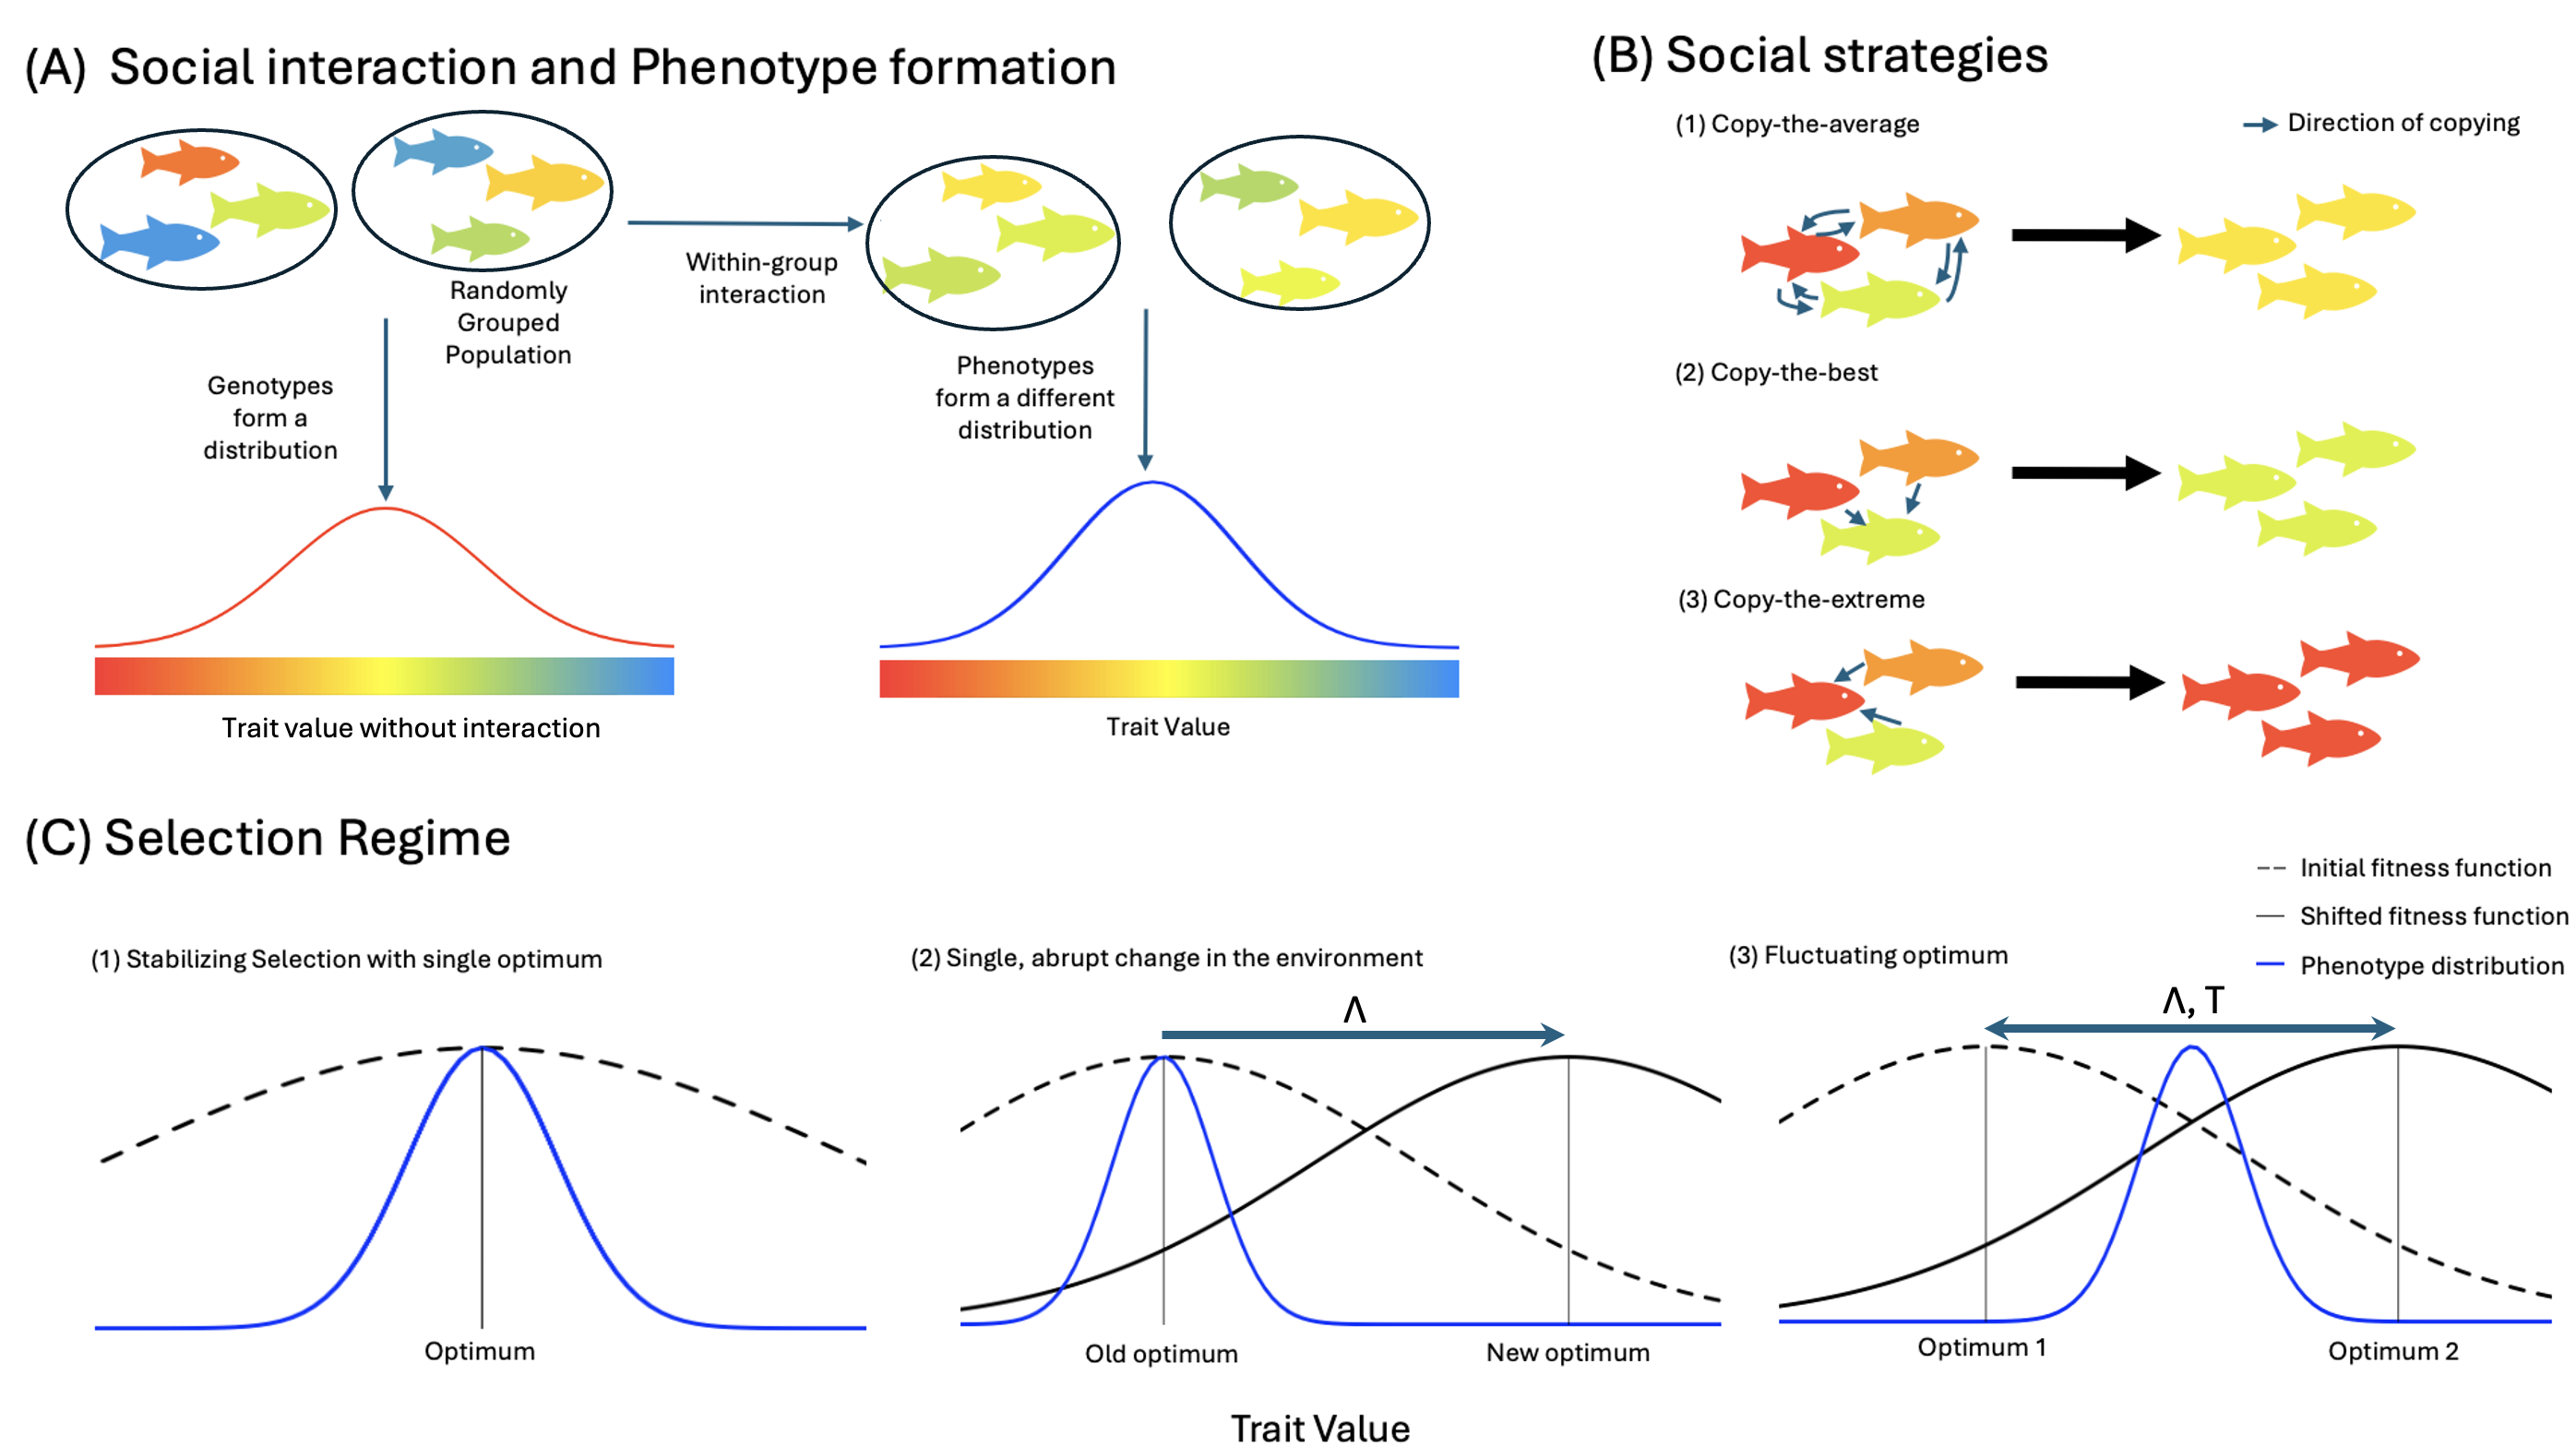
\includegraphics[width=\linewidth]{fig/model_fig.png}
    \caption{\textbf{Overview of the model structure.} (A) Within each generation, individuals are randomly partitioned into groups. Genotypes form a population-level distribution, and within-group interactions determine phenotype expression, generating a potentially different phenotype distribution. (B) Social interaction strategies modeled included copy-the-average, copy-the-best, and copy-the-extreme, which determine how do one's phenotype affected by group members. See Section \ref{sec:interaction_models}. (C) Selection regimes examined: (1) long-term stabilizing selection under a single fitness optimum, (2) a single abrupt shift in the optimum with magnitude $\Lambda$ after the stabilizing selection, and (3) a fluctuating optimum that alternates between two trait values at with period $T$ generations. Dashed and solid curves indicate the initial and shifted fitness functions, respectively; blue curves denote phenotype distributions.}
    \label{fig:model_fig}
\end{figure}

\subsection*{Social Interaction Models}\label{sec:interaction_models}
After individuals are assigned to a group of size $n$, the phenotype of each individual is calculated as Eq.~\ref{eq:z_def}. We consider three strategies that determine the value of $g_{social}$ for an individual's phenotype: copy-the-average, copy-the-best, and copy-the-extreme. These rules span a common typology in social learning theory -- majority-based, success-based, and rarity-based use of social information, respectively -- and allow us to ask whether the evolutionary consequences of social plasticity depend on \emph{which} social information individuals use, not just how strongly they use it.


\subsubsection*{Copy-the-Average}
\citep{Moore1997}'s original IGE model considered only pairwise social interactions; \citep{McGlothlin2010} extended the framework to groups of $n$ individuals, under the assumption that the focal individual is influenced by the mean phenotype of its social partners. This formulation corresponds to a form of frequency-dependent social influence in which individuals adjust their phenotype toward the tendency of the group. Conceptually, this is closely related to conformist transmission in social learning theory, where individuals disproportionately adopt the most common behavior in a population~\cite{Boyd1985}. In a binary-decision context, conformity is often represented as "copy-the-majority," pulling the group toward one of two discrete choices. However, our trait space is continuous, so there is no discrete majority category; instead, we model conformity as adjustment toward the group mean, which in turn approaches the population mean. With a symmetric trait distribution, the mean is also the most frequent phenotype, so copy-the-average provides a continuous analogue of majority-based social learning. This form of conformity-like adjustment has been documented, for example, in the convergence of foraging techniques within social groups of great tits~\cite{Aplin2014} and in individuals copying the foraging decisions of the larger of two groups in nine-spined sticklebacks~\cite{Pike2010}.

Specifically, the single-trait model from \cite{Moore1997} is extended to a group of $n$ individuals; for the $i^{th}$ individual in the group, its phenotype is

\begin{equation}
z_i = (1-\psi)g_i + \psi \frac{1}{n-1} \sum_{j \ne i}^n z_j
\label{eq:system}
\end{equation}
where $g_i$ denotes the direct genetic effect and $\psi$ the social interaction coefficient (Fig.~\ref{fig:model_fig}B1). Solving this linear system (Appendix~X) yields
\begin{equation}
z_i
=
\frac{n-1}{n-1+\psi}
\big((1-\psi)g_i \big) 
+
\frac{\psi}{n-1+\psi}
\left(
\sum_{k=1}^n g_k
\right).
\label{eq:ave_eq}
\end{equation}

Intuitively, each individual's phenotype is a weighted combination of its own direct genetic and environmental effects and the summed genetic and environmental effects of the group, with the weighting set by $\psi$ and $n$. The solution exists for $\psi \ne 1$; at $\psi = 1$ the system becomes singular. Given our definition of $\psi$ as a proportion coefficient, we keep $\psi \in [0,1)$ throughout the rest of the study.

\subsubsection*{Copy-the-Best}
Our model collapses an individual's lifetime of social interactions into a single phenotype and fitness value. However, many biological interactions instead involve repeated encounters over an individual's lifetime, such as best-of-$n$ mate choice~\cite{Janetos1980} and %TODO: find citation for nest finding in birds maybe
These repeated interactions may allow individuals to assess the success of their group mates and adjust their own phenotype accordingly, for example by copying the most successful neighbor -- a strategy known in social learning theory as payoff-biased or success-biased learning~\cite{Boyd1985,Laland2004}. To capture this dynamic, we adopt a simple model in which individuals assess the fitness of their social partners' genotypes and copy the genotype of the individual with the highest fitness (Fig.~\ref{fig:model_fig}B2). Specifically, the copy-the-best strategy for a group of size $n$ is
\begin{equation}
    z_i = (1-\psi)g_i+\psi g_{j^*} \text{ where }j^*=\arg\max_{j\in n}(W(g_j)),
\end{equation}
with the fitness function $W$ defined in Section~\ref{sec:selection_regimes}. Individuals are allowed to copy themselves, i.e., $z_{j^*}=g_{j^*}$, if they carry the best genotype in the group.

\subsubsection*{Copy-the-Extreme}
Frequency-dependent strategies usually take the form of copy-the-majority, but in some cases the minority of a group has disproportionate influence on others~\cite{Laland2004}. A recent study showed that a frequency as low as 20\% of an alternative genotype in a fire ant colony can convert the colony from monogyne to polygyne social organization~\cite{Zeng2025}. To implement an analogous strategy in a model with continuous trait values, we define "copy-the-extreme" as copying the group member whose genotype deviates most strongly from the group mean. This formulation assumes genotypes are approximately normally distributed both in the population and within groups~\cite{Lande1976}; under such a distribution, individuals far from the mean are also relatively rare, so copying the most extreme genotype captures a tendency to preferentially adopt an uncommon phenotype (Fig.~\ref{fig:model_fig}B3). The model is defined as
\begin{equation}
    z_i = (1-\psi)g_i+ \psi g_{j^*} \text{ where }j^*=\arg\max_{j\in n}(|g_j-\bar{g}|),
\end{equation}
where $\bar{g}$ is the mean genotype within the group.

Together, these three rules operationalize distinct modes of social information use that prior extensions of the IGE framework have largely collapsed into a single, undifferentiated social term. We next describe the selection regimes under which we evaluate the evolutionary consequences of each rule.

\subsection*{Evolutionary Scenarios} \label{sec:selection_regimes}
The population is simulated under three selection regimes, each implemented by changing the mean of the fitness function over time. The fitness function $W$ is assumed to be Gaussian in phenotype $z$,
\begin{equation}
W(z) = \exp\left(-\frac{(z-\mu)^2}{2\sigma^2}\right),
\label{eq:fitness}
\end{equation}
where $\mu$ is the fitness optimum and $\sigma$ determines the strength of stabilizing selection around it; fitness declines with the distance between an individual's phenotype and the optimum. This regime structure follows the evolutionary framework of \cite{Hayward2022}, in which a population under long-term stabilizing selection experiences an abrupt shift in the fitness optimum, and the dynamics of allele frequencies at a highly polygenic trait are tracked as the population adapts. We extend this framework to three scenarios: long-term stabilizing selection under a single optimum, directional selection following a single shift in the optimum, and selection under a periodically fluctuating optimum.


\subsubsection*{Stabilizing Selection}
The environment is assumed stable, with a single optimum for the trait (Fig.~\ref{fig:model_fig}C1). The population evolves under this fitness function with $\mu=0$ and $\sigma=\sqrt{2N}$ for $10N$ generations, allowing it to reach mutation-selection-drift balance, where $N$ is the population size~\cite{Hayward2022}.

\subsubsection*{Directional Selection} 
Once the population reaches mutation-selection-drift balance, the fitness optimum shifts at generation $t_s=10N$ by a magnitude $\Lambda$ (Fig.~\ref{fig:model_fig}C2). $\Lambda$ is held constant within a given comparison across social strategies and interaction coefficients; we are interested in how the trajectory of adaptation to the new optimum differs across social strategies and values of $\psi$.

\subsubsection*{Periodic Fluctuating Selection}
As an extension of the single-shift scenario, the population is instead placed under a fitness function whose optimum alternates between two values, $-\frac{\Lambda}{2}$ and $\frac{\Lambda}{2}$, with period $T$ generations (Fig.~\ref{fig:model_fig}C3). As in the stabilizing-selection scenario, the population evolves to mutation-selection-drift balance under the fluctuating optima for $10N$ generations.

\subsection*{Invasion Analysis}\label{sec:invasion_analysis}
All models presented above assumed populations that are either fully social or fully asocial. However, natural populations exhibit varying degrees of sociality~(citation), and there are many evolutionary transitions between social and solitary states~\cite{Love2026}. We therefore asked whether, and how, sociality can arise and be maintained in our model in the first place -- a question logically prior to comparing fully social and asocial populations, since a social rule that cannot invade an asocial population would never be observed to fix.

To address this, we used a rare-mutant invasion analysis: a rare social mutant is introduced into an otherwise asocial resident population, and its relative fitness determines whether the social rule can spread. For stabilizing selection, we derived the fitness of a rare social mutant relative to asocial residents analytically as a function of $\psi$ and $n$, under the assumption that each individual's genotype is drawn independently from a common normal distribution, for both the asocial resident population and the rare mutant. For asocial individuals, genotype is equal to phenotype and is therefore directly under selection. We assumed the population had reached long-term mutation--selection--drift balance under stabilizing selection, with genotypic variance $V_{res}$ and a mean equal to the fitness optimum; we set $\mu=0$, both to simplify the analysis and to match our simulation parameters. The resident population thus has a genotype distribution

\begin{equation}
    z \sim \mathcal{N}(0, V_{res}).
\end{equation}

The genotype of the rare social mutant is drawn from this same distribution, reflecting the assumption that the social trait arises by mutation within the resident population rather than by immigration. Because the social mutant is assumed rare, we consider only the case of a single social mutant per group. The mutant's phenotype is then calculated from its own genotype and the phenotypes/genotypes of the $n-1$ asocial group members, using the social rule under consideration (Section~\ref{sec:interaction_models}). Fitness for all individuals is determined using the fitness function in Eq.~\ref{eq:fitness} with $\mu=0$.

From this, we calculate the expected fitness of the social mutant, $\bar{W}_{mut}$, and of an asocial resident, $\bar{W}_{res}$, each averaged over the distribution of group compositions, and define the log invasion fitness of the mutant as
\begin{equation}
    s(\psi, n) = \ln\frac{\bar{W}_{mut}(\psi)}{\bar{W}_{res}}.
\end{equation}
If $s(\psi,n)>0$, the social mutant has higher expected fitness than the asocial resident at that value of $\psi$ and $n$ under the social rule in question, and we conclude that sociality is expected to invade. Because invasion success can depend on $\psi$ and $n$ even for a fixed social rule, we also report whether a critical value $\psi_c$ exists for each $n$, above or below which invasion outcomes change.


This analytical approach relies on the population having a well-defined equilibrium mean phenotype equal to the fitness optimum, and so applies only to stabilizing selection; we do not extend it to the single-shift (directional selection) scenario, since a one-time environmental shift lacks a stable long-run equilibrium against which invasion fitness can be defined. For the periodically fluctuating environment, we instead used simulation to test whether a social mutant could invade. We introduced a second, unlinked trait controlling whether an individual is social or asocial, represented as a single heritable tag rather than a standard diploid two-allele locus. Each offspring inherits this tag from one of its two parents, chosen at random with equal probability; consequently, offspring of two same-tagged parents always inherit that tag, while offspring of differently-tagged parents inherit either tag with 50\% probability. No mutation occurs at this locus. Individuals carrying the social tag use a fixed interaction strength $\psi=x$, with $x$ drawn from the same range of values tested in Section~\ref{sec:simulation_details}, while individuals carrying the asocial tag remain asocial.

The mutant allele was introduced at the start of a fluctuation period at a specified frequency into a population that has been under long-term fluctuating selection. Each simulation was run for up to 1000 generations (can be changed) or until the social allele was lost or fixed, whichever came first. We report results for an introduction frequency of 50\% in the main text, chosen to minimize the influence of genetic drift on invasion outcomes; results for lower introduction frequencies are given in Supplement~X.

\subsection*{Simulation Detail} \label{sec:simulation_details}

Simulations were implemented in SLiM~\cite{Haller2023} under a standard diploid Wright-Fisher model with constant population size $N=1000$ and non-overlapping generations. The genetic architecture follows the Lande-type model of \cite{Hayward2022}, with a maximum of $L_{MAX}=10000$ mutable loci. Mutations arise at rate $U=0.03$ per gamete per generation, with effect size magnitude $|a|$ drawn from a Rayleigh distribution with scale parameter $\sigma=1$.

Within each generation, the simulation proceeds as follows: (1) individuals are randomly partitioned into groups of size $n$; (2) each individual's phenotype $z_i$ is computed from Eq.~\ref{eq:z_def} according to the social interaction rule in effect (Section~\ref{sec:interaction_models}); (3) individual fitness is evaluated from $W(z_i)$ (Eq.~\ref{eq:fitness}); (4) mating and reproduction occur, treating the population as panmictic -- grouping affects only phenotype expression, not mate choice or offspring production. Group assignment is re-randomized each generation.

We varied the social interaction coefficient $\psi \in \{0, 0.2, 0.5, 0.8\}$, where $\psi=0$ corresponds to the asocial control population, and group size $n$ across all integer divisors of $N=1000$ between 2 and 100 such that there is no remainder individuals. Simulation in the main text are shown with $n=8$ with additional results in Supplement~X. For directional selection, we tested three shift magnitudes, $\Lambda \in \{20, 40, 60\}$. For the fluctuating-environment scenario, we instead swept $\Lambda$ and the fluctuation period $T$ over broader grids, $\Lambda \in \{10, 20, \ldots, 100\}$ and $T \in \{20, 40, \ldots, 180\}$ generations. Full parameter values, along with the rationale for the chosen ranges, are provided in Supplement~X. Each combination of parameter is run for 1000 replicates (TODO: run more replicates).



\section*{Result}
\subsection*{Stabilizing Selection}
\begin{figure}
    \centering
    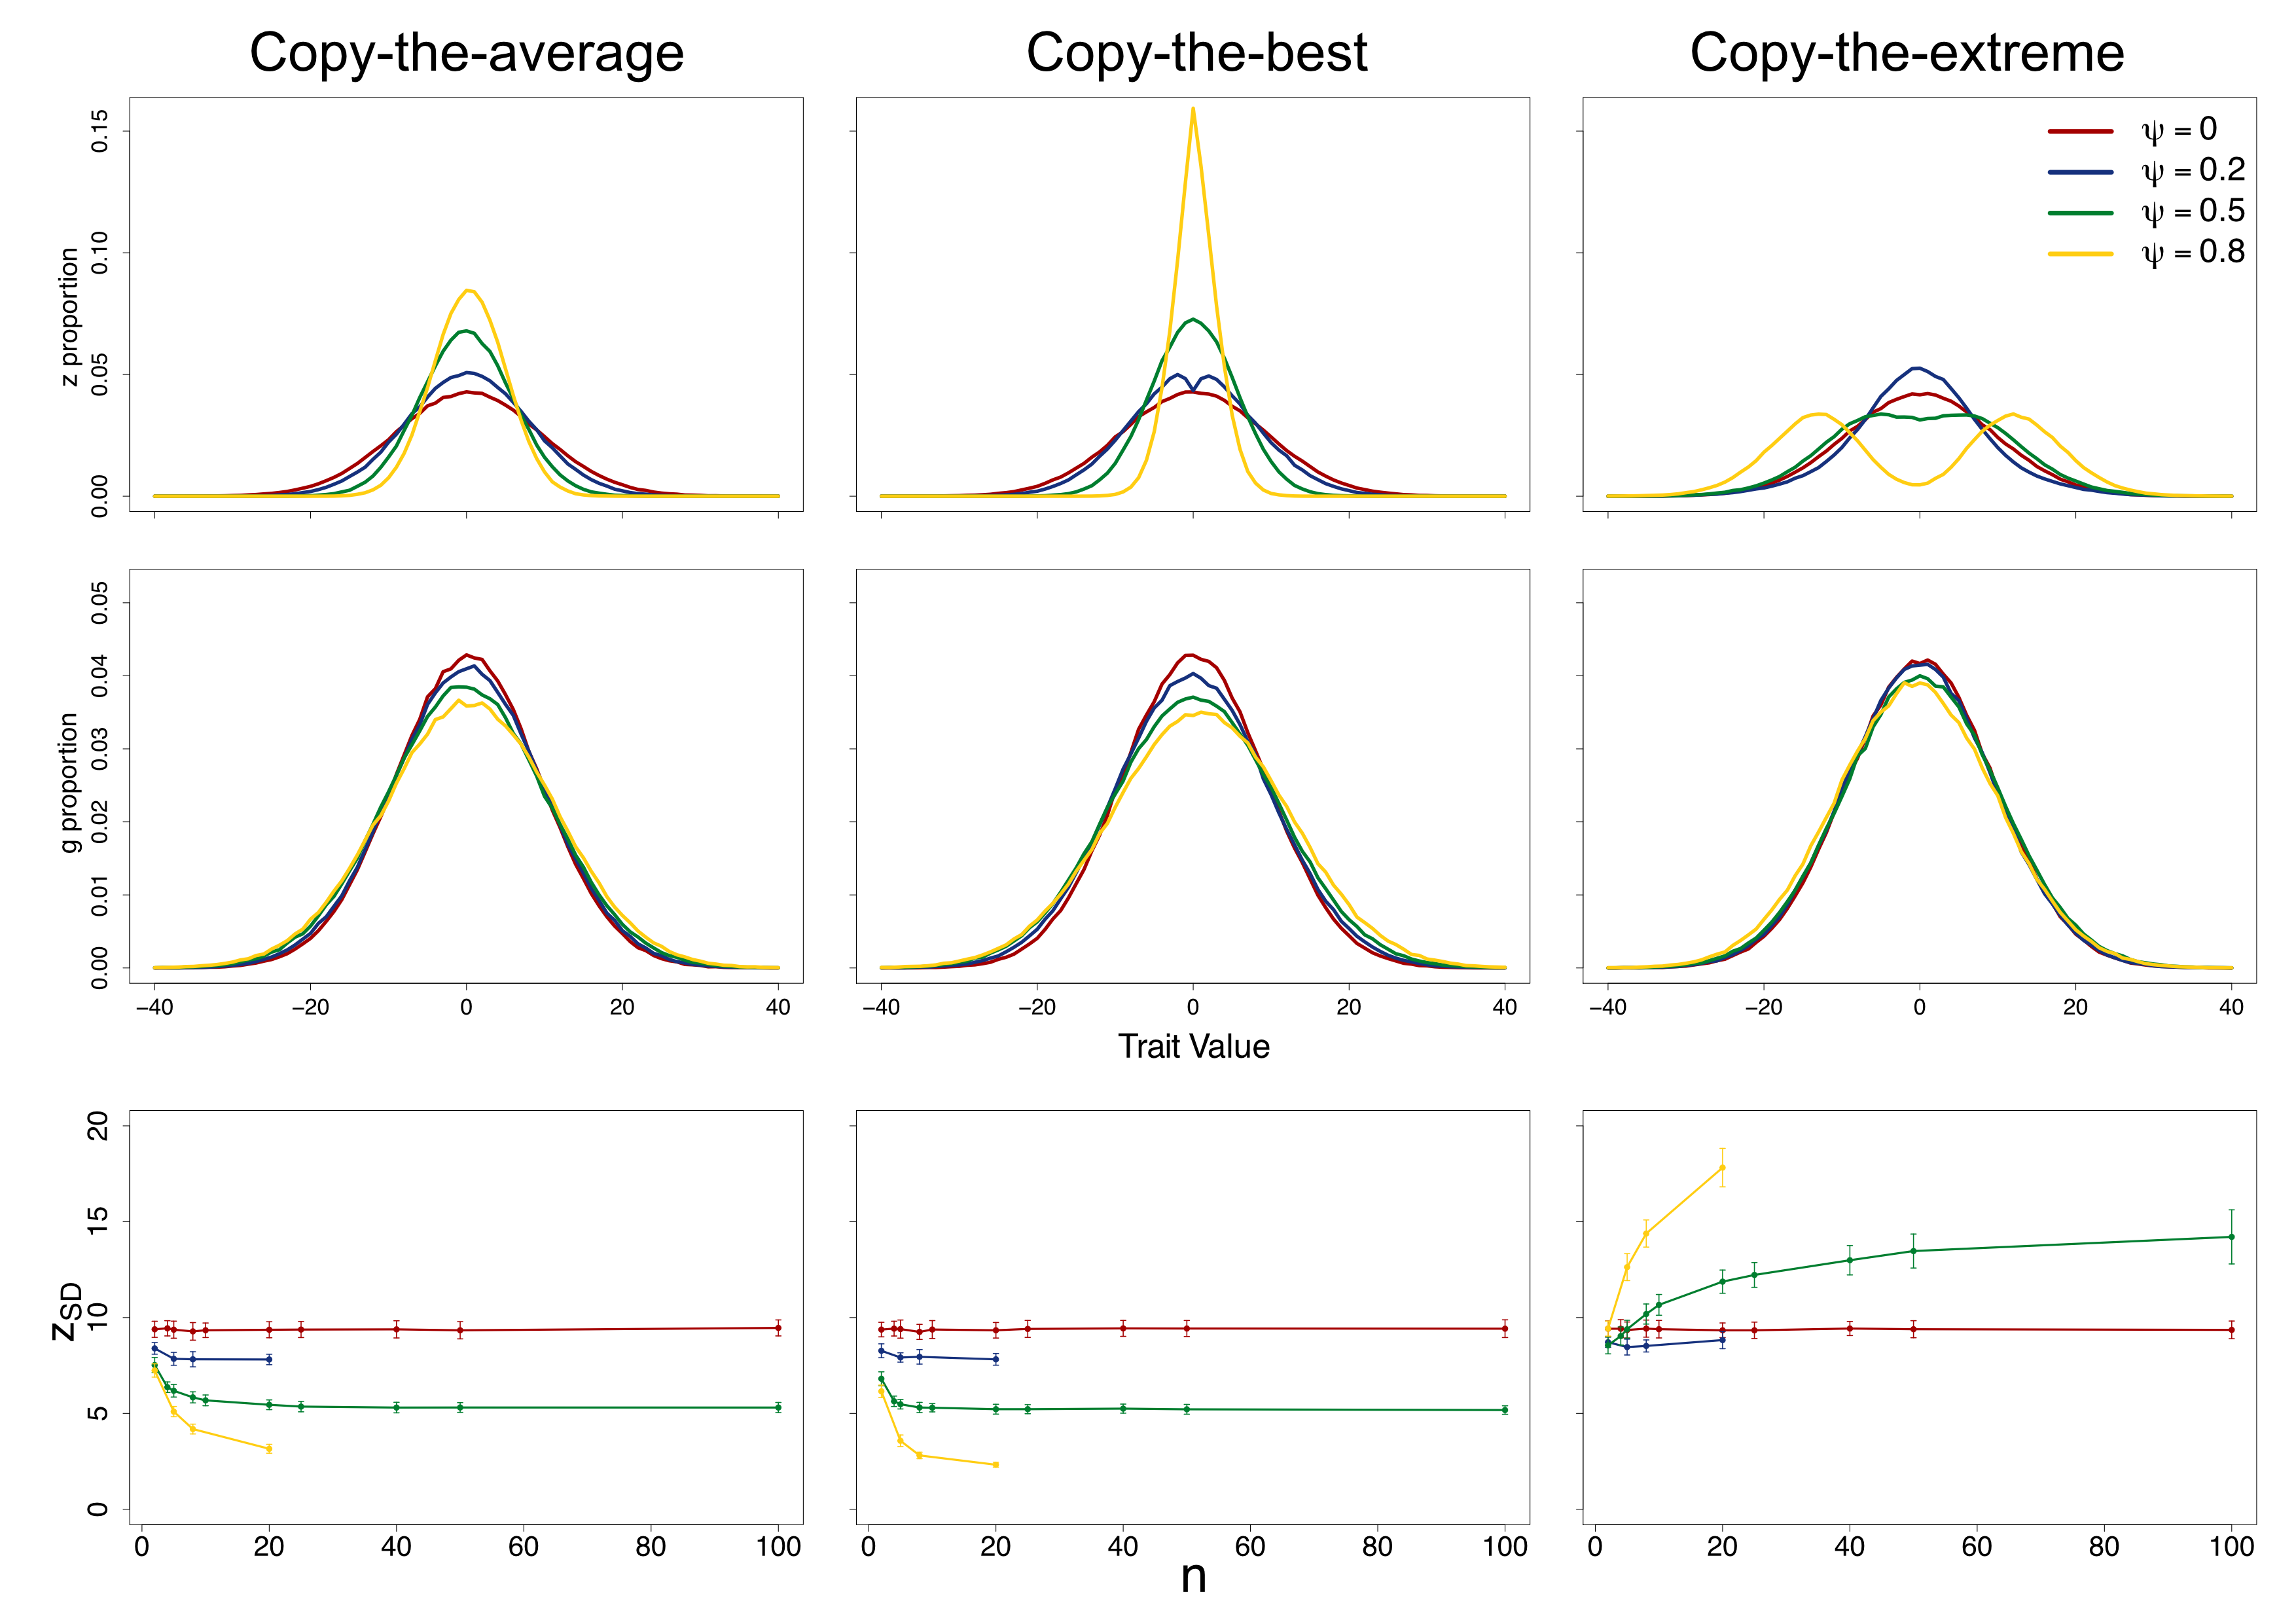
\includegraphics[width=\linewidth]{fig/stab/stab_sel.png}
    \caption{\textbf{Effect of social learning mechanisms, $\psi$, and $n$ on population's statistics under stabilizing selection.} $n=8$ for the top two rows. \textbf{Top row:} Phenotype distribution of different values of $\psi$. For both copy-the-average and copy-the-best model, increasing in $\psi$ always leads to decrease in phenotypic variance. Copy-the-best has slight bimodality for low $\psi$, though the pattern is not significant (see Supplement TODO). Variance for Copy-the-extreme decreases first before increasing as $\psi$ increases, eventually leads to bimodal phenotypic distribution.
    \textbf{Middle row: }Genotypic distribution for different $\psi$. The genotypic variance always increase with $\psi$ regardless of the shape of the phenotypic distribution, though the change is small compare to the change in phenotypic distribution as $\psi$ increasing. 
    \textbf{Bottom row: }Standard deviation (SD) of the phenotypic distribution as a function of group size $n$. For copy-the-average and copy-the-best models, as group size increases, the phenotypic variance further decreases. For copy-the-extreme, higher $n$ leads to a larger distance between modes for larger $\psi$, thus SD is elevated. In all cases, the change in SD decreases as $n$ increases. (TODO: fill the remaining data points)}
    \label{fig:stabl_sel_1}
\end{figure}
We first examined how the three social interaction rules alter the genotype-phenotype relationship under long-term stabilizing selection (Fig.~\ref{fig:stabl_sel_1}). In the absence of environmental change, all populations evolved around a single fitness optimum, but the shape of the resulting phenotypic distribution depended strongly on both the social rule and the interaction strength $\psi$. Across all three rules, the underlying genotypic distributions remained approximately unimodal and centered near the optimum, indicating that social interaction primarily reshaped phenotype expression rather than producing large shifts in the population mean genotype. The resulting phenotypic distributions, however, differed substantially among the three rules.

Under copy-the-average, increasing $\psi$ reduced phenotypic variance (Fig.~\ref{fig:stabl_sel_1}) and slightly increased genotypic variance (TODO: test the difference in variance (supplement)). As individuals placed greater weight on the mean phenotype of their social partners, phenotypes became increasingly concentrated around the population mean. This effect was strengthened by larger group size: as $n$ increased, the social value $g_{social}$ approached the population mean more closely, producing stronger compression of the phenotypic distribution. Copy-the-average thus acted as a stabilizing social mechanism, reducing among-individual phenotypic variation while leaving the genotypic distribution comparatively broad.

A similar reduction in phenotypic variance was observed under copy-the-best for small-to-medium $\psi$ ($\psi\leq0.5$) and considerably stronger at higher $\psi$. As $\psi$ increased, phenotypes became concentrated near the optimum, producing a narrow peak in the phenotypic distribution similar to that of copy-the-average. This occurs because the copied genotype is chosen based on the highest fitness within the group, which under stabilizing selection corresponds to the genotype closest to the optimum; social influence under copy-the-best therefore pulls phenotypes directly toward the fitness optimum. Although the genotypic distribution showed only modest changes with increasing $\psi$, the phenotypic distribution narrowed substantially, indicating that copy-the-best can generate adaptive phenotypic change without a corresponding degree of genetic change. Because the phenotypic distributions of copy-the-best and copy-the-average appear visually similar for $\psi \le 0.5$, we do not draw a strong distinction between the two rules in this regime without a formal statistical comparison; (TODO: run variance comparison (supplement)) %TODO: run variance comparison (e.g. Levene's test or bootstrap CI on variance) across replicates for psi <= 0.5, or soften further if not run.

Copy-the-extreme, by contrast, produced a qualitatively different, non-monotonic pattern. At low $\psi$, phenotypic variance was counterintuitively slightly reduced relative to the asocial baseline: the extreme group member's genotype can be on the same or opposite side of the distribution than the copier, and the pull from the opposite side is greater than that from the same side under the same $\psi$. When $\psi$ is small, such force is more effective than the pulling force from $\psi$, thus more individuals are concentrated around the distribution mean (TODO: if this explanation is not clear, I can add a supplement section for this). As $\psi$ increased further, the phenotype distribution grew increasingly broad and eventually bimodal, reflecting that individuals' phenotypes are dominated by extreme group member whose genotype is likely far away from the optimum. This effect intensified with group size, since larger groups are more likely to contain individuals with more extreme genotypes (Fig \ref{fig:stabl_sel_1}). As a result, copy-the-extreme amplified phenotypic variance even though the underlying genotypic distribution remained approximately normal. 

Together, these results show that the evolutionary consequences of social behavior under stabilizing selection depend strongly on the rule by which social information is used. Copy-the-average and copy-the-best both reduce phenotypic variance, but through different mechanisms: copy-the-average pulls individuals toward the group mean, whereas copy-the-best pulls individuals toward the locally highest-fitness genotype. Copy-the-extreme, by contrast, can transform a unimodal genotypic distribution into either a unimodal or a bimodal phenotypic distribution depending on the strength of interaction $\psi$, demonstrating that social interaction can generate phenotypic structure not directly present in the underlying genetic variation.


\subsection*{Directional Selection}
\begin{figure}
    \centering
    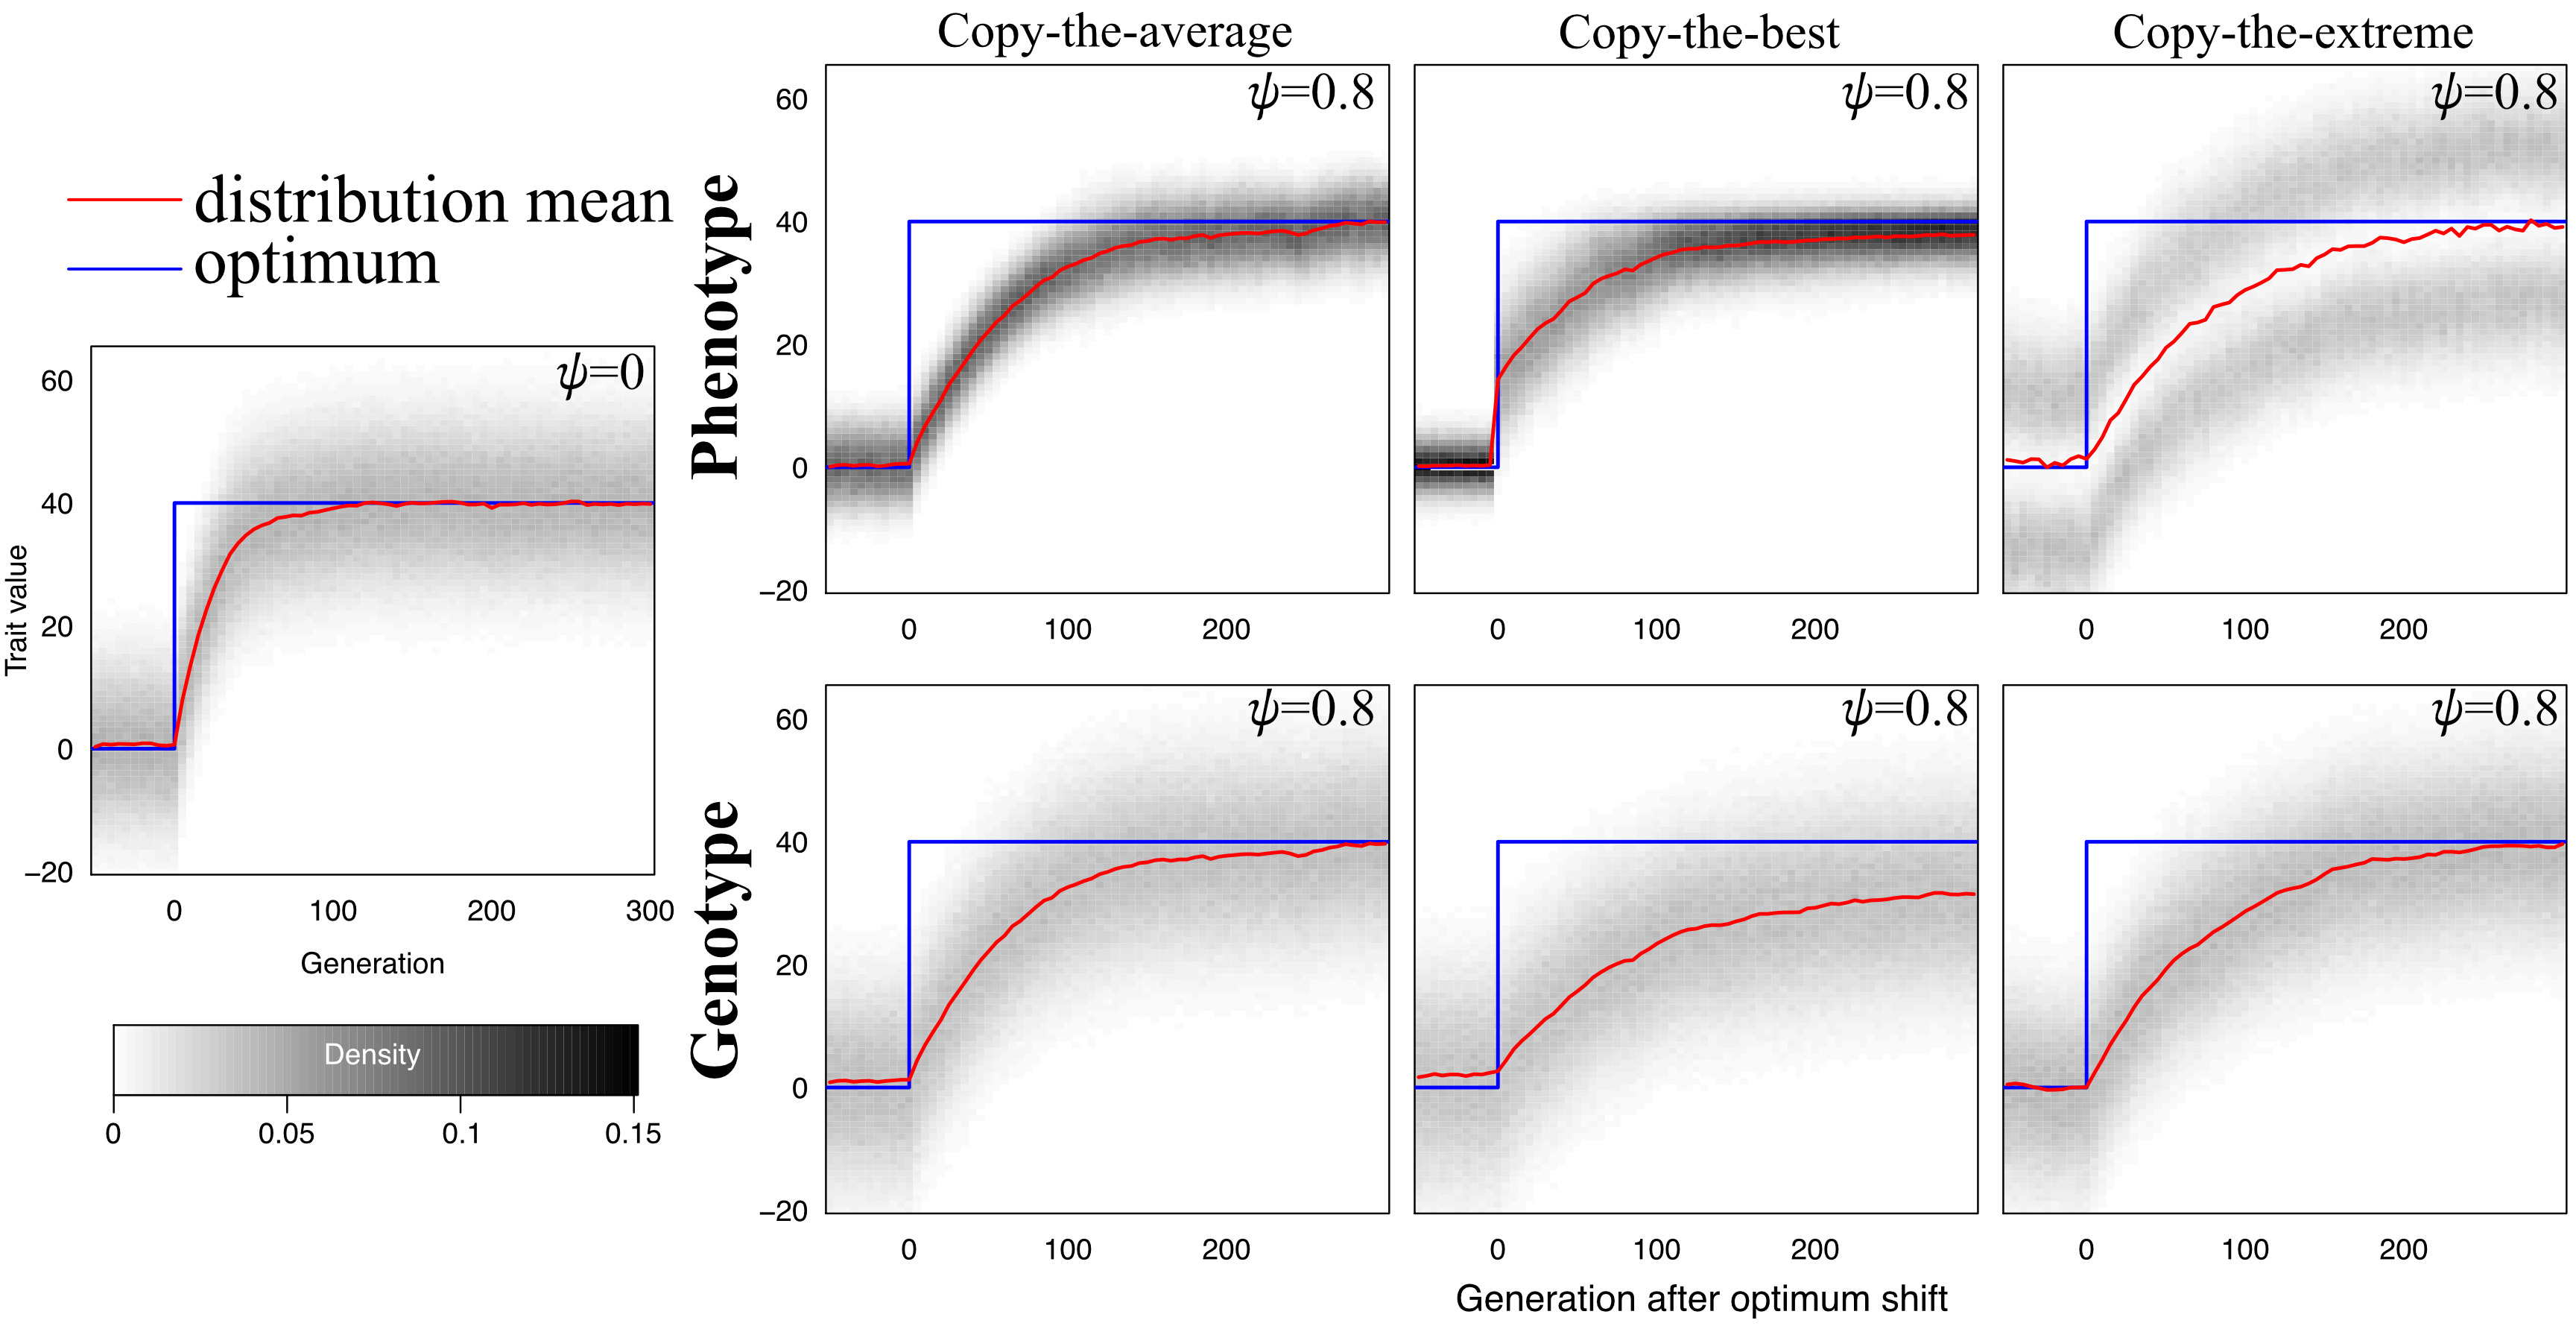
\includegraphics[width=\linewidth]{fig/direc/geno_pheno_dist_direc.png}
    \caption{\textbf{Population adapts to the new optimum after long-term stabilizing selection.}
    Distributions of trait values through time are shown for the asocial case, $\psi = 0$ (left), and three social strategies at $\psi = 0.8$, with group size $n = 8$ and optimum shift amplitude $\Lambda = 40$ (right). The blue line is the environmental optimum and the red line indicates the mean of the plotted distribution. Immediately after the optimum shifts, the copy-best strategy produces a rapid phenotypic jump toward the new optimum, followed by a slower approach to the optimum. In contrast, copy-extreme maintains a bimodal phenotypic distribution during adaptation. Overall, although all social strategies eventually phenotypically track the new optimum, adaptation is slower than in the asocial population.}
    
    % Colored lines represent different interaction strength, $\psi$, with thin lines showing individual simulations and thick lines showing replicate means. $\Lambda=40$ for all simulations shown. \textbf{Top row: } Distance between $\bar{z}$ and the current fitness optimum. After the change at the 10000 generation, all population using copy-the-average and copy-the-extreme is $\Lambda$ unit away from the new optimum. Copy-the-best shows instant phenotypic response, generating $\bar{z}$ that's much closer to the optimum than asocial population ($\psi=0$). Such change in phenotype increases as $\psi$ increases. Inset: mean genotype $\bar{g}$ vs mean phenotype $\bar{z}$ over time. Lighter color is earlier in adaptation. For copy-the-average, $\bar{g}$ tracks $\bar{z}$ perfectly, which is why there's only the yellow points. The tracking is more noisier for copy-the-extreme. Copy-the-best show the largest gap between $\bar{g}$ and $\bar{z}$ earlier in the adaptation and only gets smaller when the phenotype is close to the new optimum. (TODO: change to no replicate lines)
    % \textbf{Bottom row: } The decay constant fitted to the line of $\bar{z}$ to new optimum as a function of $n$. As $n$ increases, the rate of approaching the new optimum becomes slower. The change in adaptation rate decreases as $n$ get large, though which $n$ does the plateau reached depends on $\psi$.} 
    \label{fig:direc_sel_1}
\end{figure}

We next asked how the three social interaction rules affect adaptation following an abrupt environmental shift. After the population reached mutation-selection-drift balance under stabilizing selection, the fitness optimum was shifted by magnitude $\Lambda$, and we tracked the population phenotypic and genotypic distribution through time (Fig.~\ref{fig:direc_sel_1}). In Fig.~\ref{fig:direc_sel_1} we only show $\psi=0.8$ for social populations; more results on different $\psi$ are in Supplement~X (TODO).

In the asocial baseline ($\psi=0$), the population adapted gradually toward the new optimum through genetic evolution alone. Copy-the-average and copy-the-extreme showed no immediate phenotypic response at the time of the shift: populations remained approximately $\Lambda$ units from the new optimum immediately afterward, with a gradual, approximately exponential approach thereafter. Increasing $\psi$ slowed this recovery, especially at larger group sizes (TODO: Supplement~X, effect of $n$). Under copy-the-average, stronger social influence kept individuals closer to the group mean, damping the expression of phenotypic deviations in the direction of the new optimum. Both rules preserved the same distributional shape observed under stabilizing selection: copy-the-average produced a narrower, unimodal phenotypic distribution than the asocial population, while copy-the-extreme retained its bimodality at high $\psi$ (Fig.~\ref{fig:direc_sel_1}).

Copy-the-best showed a qualitatively different short-term response. Immediately after the shift, populations with stronger social influence produced mean phenotypes closer to the new optimum than the asocial baseline. This occurred because the highest-fitness genotype within each group was already biased toward the new optimum, allowing individuals to express phenotypes closer to the new selective target before the population mean genotype itself had evolved substantially. The magnitude of this response increased with both $\psi$ and group size $n$, reflecting the larger genetic variance maintained under stabilizing selection: a larger genetic reservoir means more low-fitness individuals are retained prior to the shift, and these individuals became the high-fitness group leaders once the optimum moved. Such effect plateaued as $\psi$ and $n$ further increases. Copy-the-best thus generated an immediate adaptive plastic response whose magnitude depended on both interaction strength and group size (TODO: Supplement~X, jump heatmap). Phenotypic variance also increased during this initial jump relative to stabilizing selection (TODO: report variance comparison, Supplement~X).

This short-term benefit, however, did not translate into faster long-term adaptation. After the initial phenotypic jump, the phenotypic and genotypic distributions of populations with $\psi \neq 0$ approached the optimum more slowly than the asocial baseline, and this slowing increased with both $\psi$ and $n$ (TODO: Supplement~X, decay constant plot). The gap between mean genotype and mean phenotype narrowed gradually as genetic evolution caught up with phenotypic evolution, reflecting relaxed selection on phenotype as the population approached the new optimum. Notably, this gap did not fully close even once the population's mean phenotype had reached the new optimum: because selection on phenotype relaxes as the optimum is approached, the residual gap between genotype and phenotype persisted longer, slowing further genetic convergence (TODO: Supplement~X, genotype--phenotype gap over time; longer simulation to observe the averaged number of generations for the gap to close, if feasible). In other words, copy-the-best produces adaptive plasticity in the short term while slowing genetic tracking of the new optimum over longer timescales, and this trade-off depends on both $\psi$ and $n$.

Copy-the-extreme also slowed adaptation after the shift, but through a different route. Like copy-the-average, it produced no strong adaptive jump toward the new optimum; instead, stronger social influence increased phenotypic spread and introduced noisier tracking between genotype and phenotype, reducing the efficiency with which selection acted on genetic values aligned with the new optimum. As with the other rules, increasing group size further slowed the rate of adaptation, though this effect weakened at larger $n$, suggesting a plateau in the influence of group size.

Overall, the three social rules altered both the immediate phenotypic response to environmental change and the subsequent rate of adaptation. Copy-the-best was unique in producing a rapid adaptive shift in phenotype immediately after the environment changed, accompanied by a persistent mismatch between the genotypic and phenotypic distributions during adaptation. All three rules tended to reduce the long-term rate of approach to the new optimum. 


\subsection*{Fluctuating Selection}

\begin{figure}
    \centering
    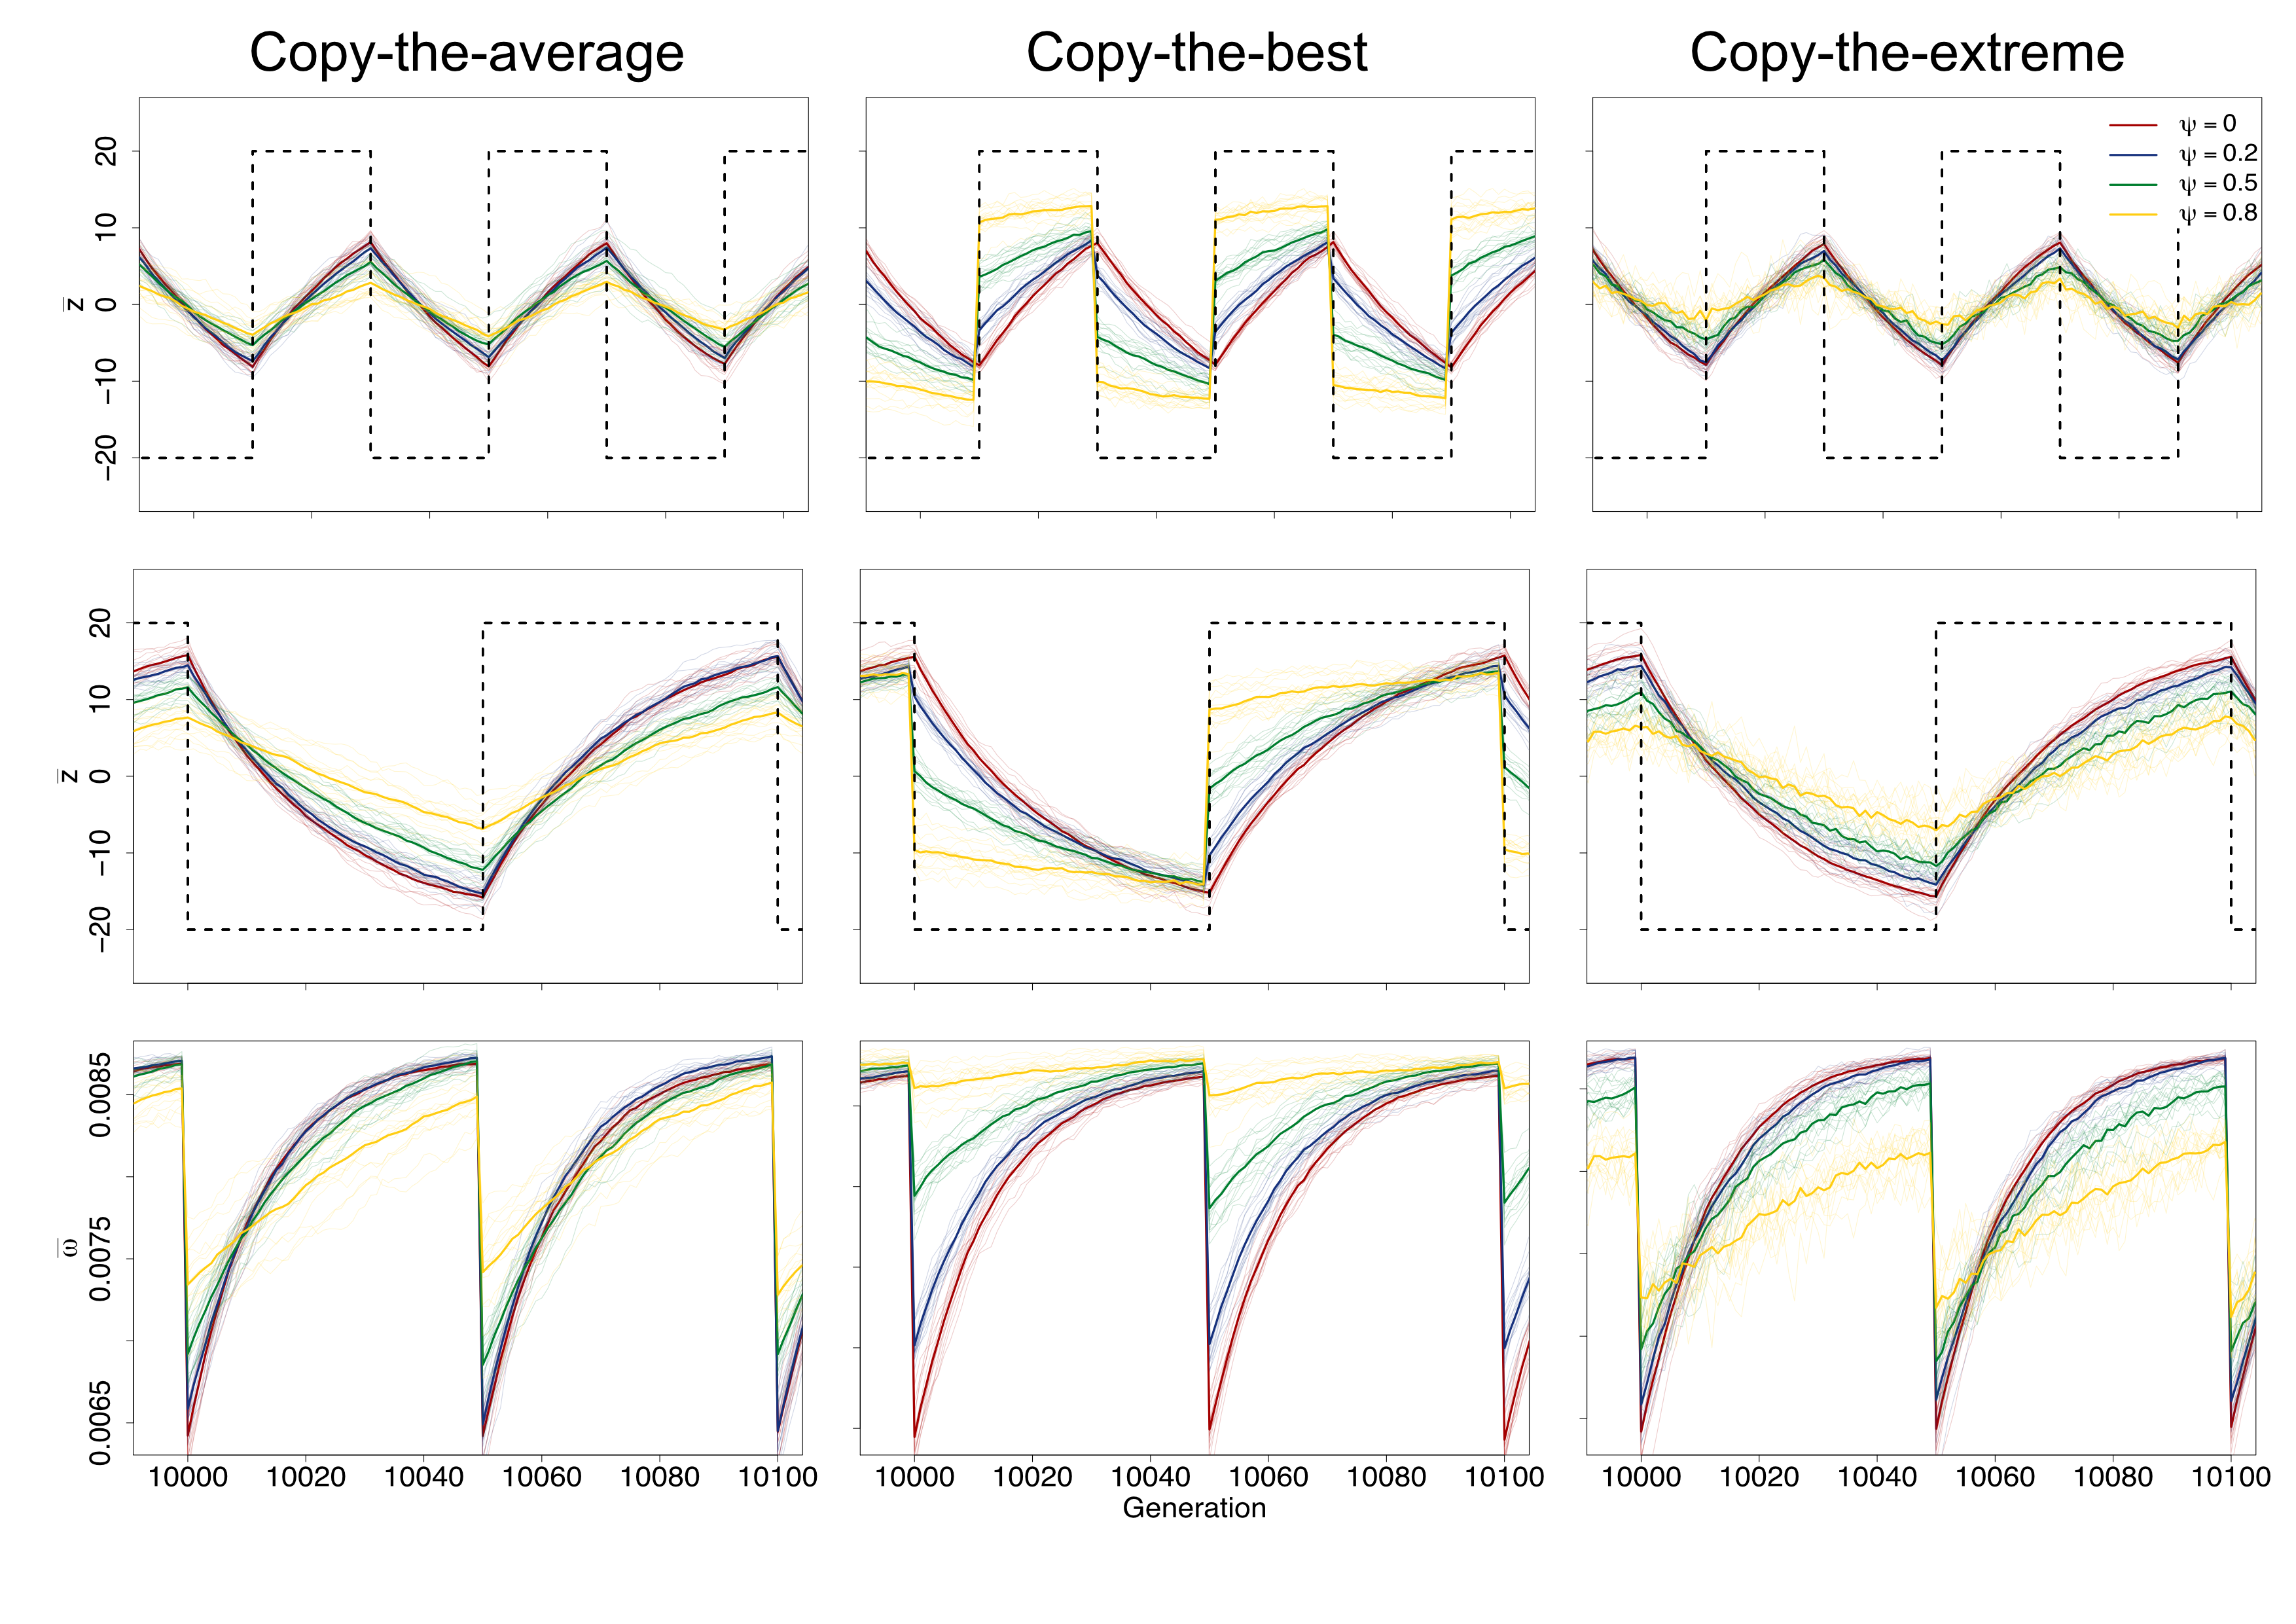
\includegraphics[width=\linewidth]{fig/fluc/fluc_env_main.png}
    \caption{\textbf{Models track the optimum differently under a periodically fluctuating environment.} Population responses are shown under three social learning rules: copy-the-average, copy-the-best, and copy-the-extreme. Black dashed lines indicate the environmental optimum. \textbf{Top and middle row:} The phenotypic mean of the population over time with different period $T$. $T=40$ generations and $T=100$ generations for the top row and middle row, respectively. \textbf{Bottom row:} population mean fitness $\bar{\omega}$ for the middle row.}
    \label{fig:fluc_env_main}
\end{figure}

\begin{figure}
    \centering
    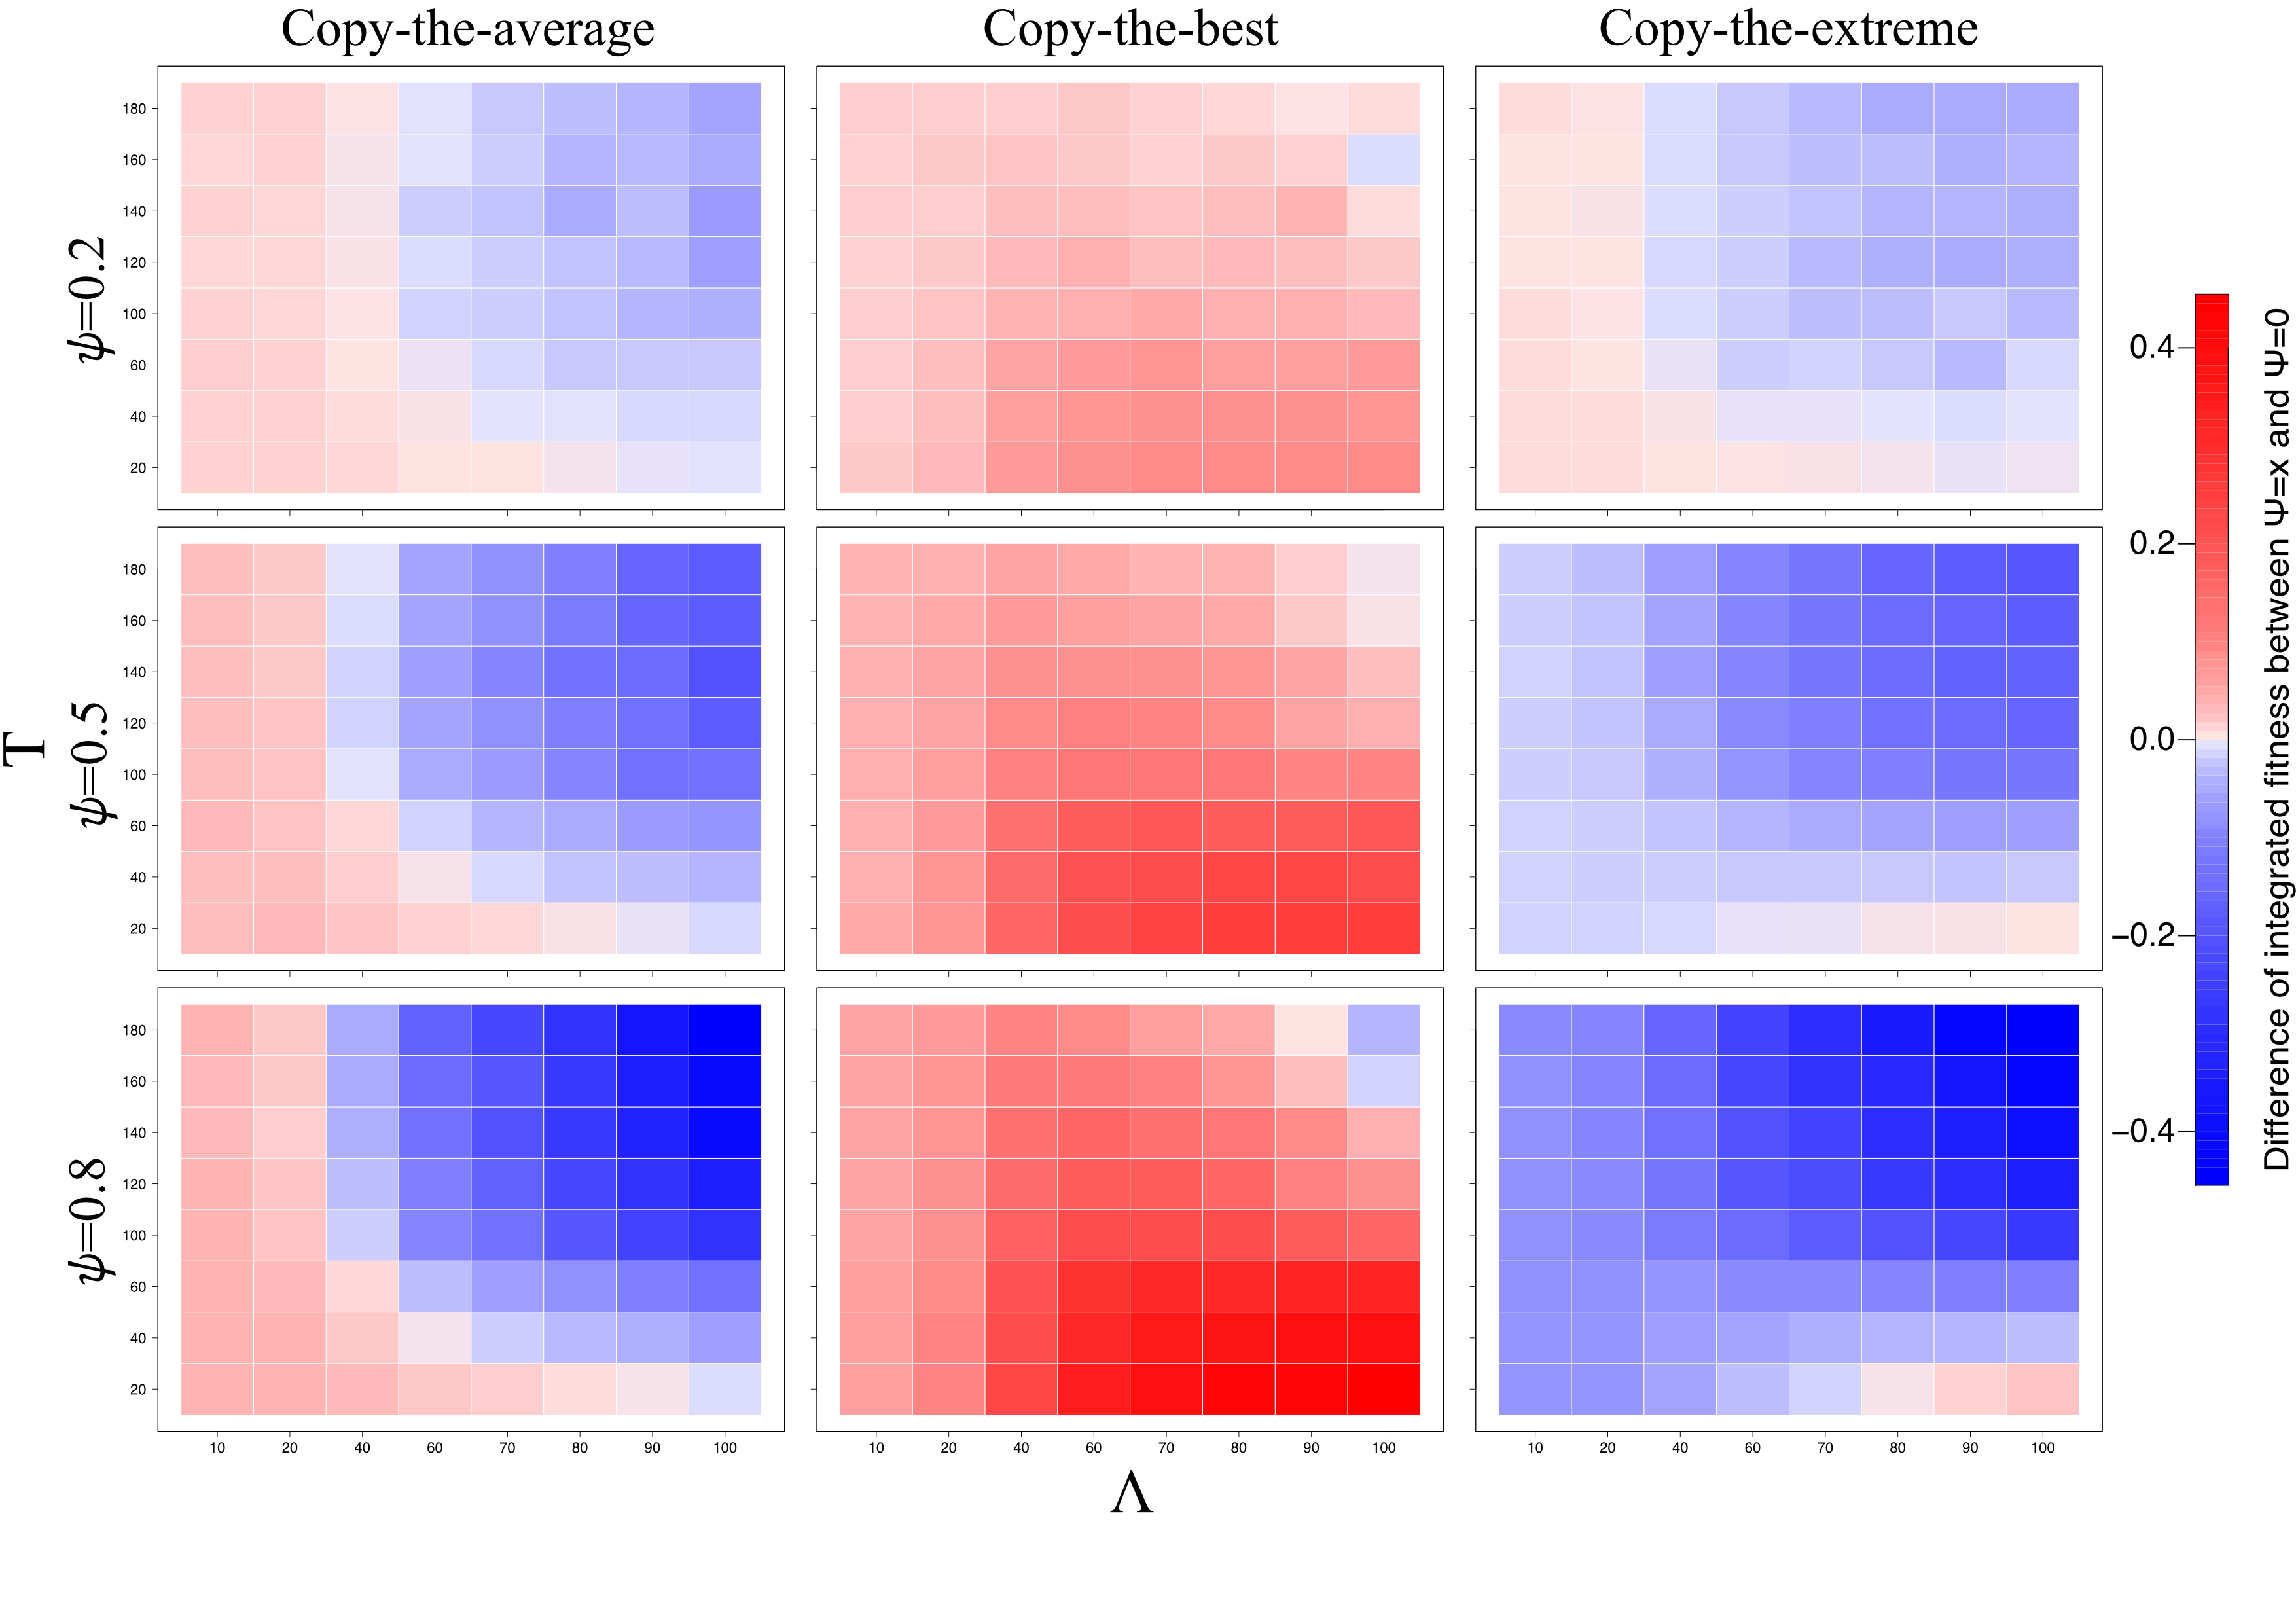
\includegraphics[width=\linewidth]{fig/fluc/integrated_fitness_fluc_env.png}
    \caption{\textbf{Integrated fitness differences across fluctuating environments.} Each tile shows the replicate-averaged difference in cumulative mean fitness between a social population and the corresponding asocial baseline, $\psi=0$, after summing $\bar{\omega}$ across 300 generations. Red indicates that social behavior produced higher integrated fitness than the $\psi=0$ baseline, while blue indicates lower integrated fitness. Copy-the-best generally improves cumulative fitness across much of the parameter space, especially at larger $\psi$ and moderate shift sizes. Copy-the-average and Copy-the-extreme can yield higher cumulative fitness when environmental shifts are small or infrequent, though the reduction in fitness is more severe otherwise.}
    \label{fig:fluc_env_fit}
\end{figure}

As an extension of previous two types of selections, we examined how populations respond when the fitness optimum fluctuates periodically between two trait values. In small amplitude $\Lambda$, the selection is similar to stabilizing selection in that the optimum is easily trackable without prolong period of adaptation. As $\Lambda$ increases, there is higher and higher selective pressure from directional selection, but the direction of selection would repeatedly reverses before the population can stabilize at either optimum. We therefore asked whether social interaction improves or worsens tracking of a moving optimum, and whether this depends on fluctuation frequency, shift size, group size, $\psi$, and social rule.

Across all three rules, populations lagged behind the changing optimum (Fig.~\ref{fig:fluc_env_main}), but the magnitude and direction of this lag depended on the rule. Under copy-the-average, increasing $\psi$ reduced the amplitude of phenotypic tracking. This damping could be beneficial when environmental changes were frequent (small $T$) or small ($\Lambda$): a population that adapts more slowly toward one optimum remains closer to the other optimum once the environment shifts again, relative to the faster-adapting asocial population. However, this benefit of lagging behind lasted only a few generations before the asocial population outperformed all social populations. Thus, although copy-the-average can have a fitness advantage over the asocial baseline, this advantage depends on how the environment fluctuates, namely on $T$ and $\Lambda$.

Given that in fluctuating selection, there is no stable point where we can compare the performance/fitness across parameter values and social rules (Fig \ref{fig:fluc_env_main}). To characterize the dependence between population fitness and $T$ and $\Lambda$, we integrated mean fitness $\bar{\omega}$ over 300 generations for each simulation and examined how $T$ and $\Lambda$ jointly determine whether a given parameter combination outperforms the asocial population (Fig.~\ref{fig:fluc_env_fit}). For copy-the-average, overall fitness was higher than the asocial baseline when $T$ or $\Lambda$ was small, and declined as either increased; larger $\psi$ produced a greater fitness benefit at low $T$ or $\Lambda$, but also a more severe decline as either parameter grew. The higher fitness at low $T$ or $\Lambda$ does not reflect better optimum tracking by the social population -- rather, the social population lags behind the old optimum and is therefore closer to the new value, and has higher instantaneous fitness, at the moment the environment shifts again.

Copy-the-best produced a qualitatively different form of tracking. At each environmental shift, the abrupt phenotypic response allowed populations to move toward the new optimum more quickly than genetic change alone would predict (Fig.~\ref{fig:fluc_env_main}). However, the slower adaptation that followed this plastic response limited optimum tracking when fluctuations were less frequent (larger $T$): the asocial baseline was able to catch up over time, and its $\bar{z}$ came closer to the optimum than that of the social populations. Whether copy-the-best was beneficial therefore depended on $T$ and $\Lambda$ jointly -- the more closely a fluctuating environment resembled a single shift, the more likely copy-the-best was to be maladaptive, whereas frequent fluctuations favored copy-the-best because the benefit of the initial plastic response outweighed the cost of slower subsequent adaptation.

Consistent with this, integrated fitness for copy-the-best was generally higher than the asocial baseline across much of the parameter space, especially at moderate shift sizes and higher $\psi$ (Fig.~\ref{fig:fluc_env_fit}), reflecting phenotypes' ability to respond plastically to the currently favored direction of selection. This advantage diminished as $T$ or $\Lambda$ moved away from moderate values: for small $\Lambda$, the asocial baseline tracked the optimum closely enough that its integrated fitness approached that of the social population, while for large $\Lambda$ and $T$, the social population became maladaptive as the cost of slower adaptation outweighed the benefit of the initial plastic response.

Copy-the-extreme generally reduced tracking accuracy in fluctuating environments and behaved similarly to copy-the-average: because individuals copied the most extreme genotype in the group rather than the genotype closest to the current optimum, social influence often pushed phenotypes away from the optimal value. This effect was helpful at frequent fluctuation with large amplitude when the two modes of the phenotypic distribution covered the two optima value better than asocial population tracking them. However, the bimodality was especially costly at high $\psi$ for any other combination of $T$ and $\Lambda$, where integrated fitness was substantially lower than the asocial baseline. Under mild environmental conditions -- small shifts and frequent fluctuations -- copy-the-extreme produced weakly positive or near-neutral effects, but its overall effect was more often negative than that of copy-the-best.

\subsection*{Social Invasion} 

\begin{figure}
    \centering
    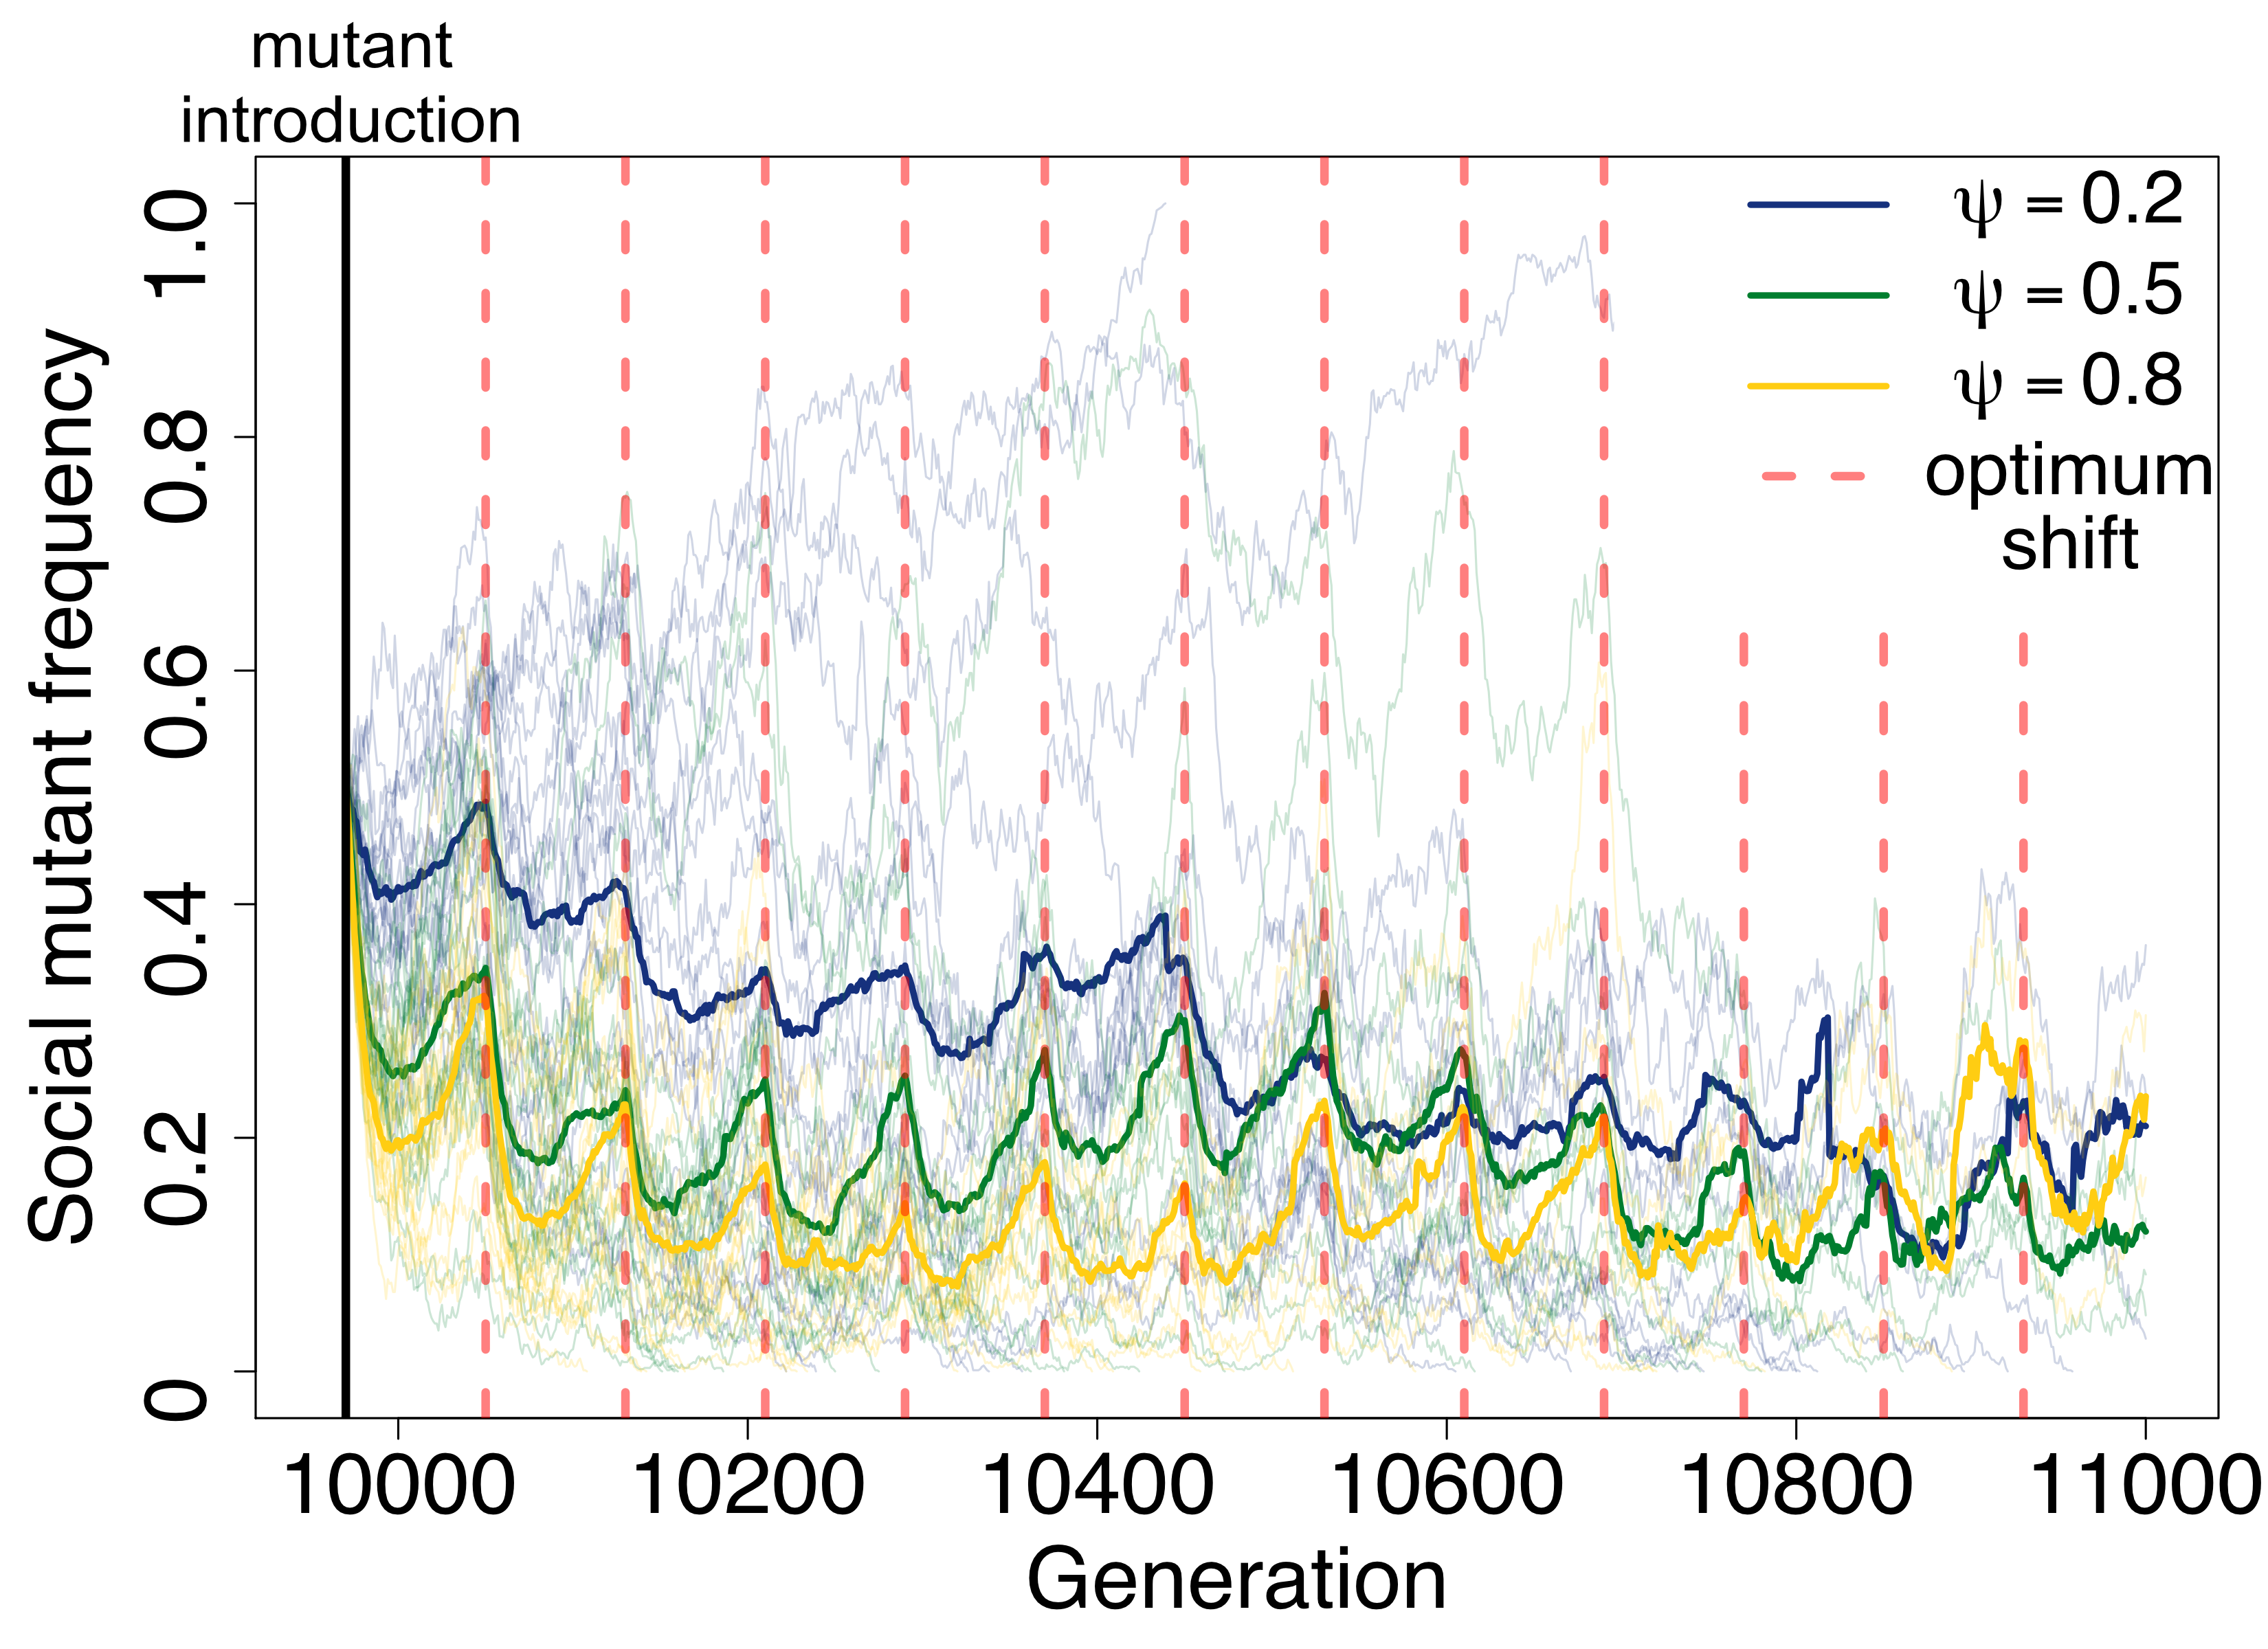
\includegraphics[width=\linewidth]{fig/fluc/fluc_ave_invasion.png}
    \caption{\textbf{Social mutants fluctuates in fluctuating environment for copy-the-average strategy} Social mutants of $\psi=x$ were introduced at 50\% frequency with $T=160$ generations and $\Lambda=100$. Social mutants are under purifying selection when the environment optimum shifted recently. As the population moves closer to the new optimum, sociality is beneficial and increase in frequency. }
    \label{fig:fluc_invasion}
\end{figure}

For stabilizing selection, we derived the invasion fitness of a rare social mutant relative to an asocial resident population (Supplement~X). We showed that the only condition necessary for successful invasion, i.e., $s(\psi,n)>0$, is $V_{mut}(\psi,n) < V_{res}$, where $V_{mut}$ is the expected variance of the mutant's phenotype. Intuitively, if the mutants can be closer to the fitness optimum, which is also $\mu$, they will have higher fitness than asocial individuals. For copy-the-average and copy-the-best, $V_{mut}(\psi,n) < V_{res}$ held for all values of $\psi$ and $n$, with a monotonic decrease in $V_{mut}$ as $\psi$ increased -- consistent with our simulation results (Fig.~\ref{fig:stabl_sel_1}). Any strength of sociality under these two rules is therefore expected to invade, for any group size $n$.

For copy-the-extreme, by contrast, our simulation results suggested a nonmonotonic relationship between $V_{mut}$ and $\psi$ (Fig.~\ref{fig:stabl_sel_1}), implying a critical value $\psi_c$ below which invasion succeeds. Solving $s(\psi,n)>0$ confirmed this, yielding

\begin{equation}
    \psi_c(n) \approx \frac{2}{1+2\ln(n-1)}.
\end{equation}

Notably, the invasion threshold for copy-the-extreme depends only on group size $n$, not on the amount of standing genetic variation in the resident population. Intuitively, increasing either $\psi$ or $n$ strengthens the social contribution to phenotype ($\psi g_{social}$ in Eq.~\ref{eq:z_def}) and broadens the phenotypic distribution; invasion succeeds only when $\psi$ and $n$ keep this distribution narrower than that of the asocial population ($V_{mut}(\psi,n) < V_{res}$). (TODO: plot for the density of the center bin of the distribution as a function of $\psi$ for various group size in supplement)

For the fluctuating-environment scenario, we tested invasion under copy-the-best and copy-the-extreme for all values of $n$. Social mutants under copy-the-best always fixed in the population, with faster fixation at higher $\psi$. Under copy-the-extreme, high-$\psi$ social mutants consistently failed to invade for (TODO: values of $n$ tested), while mutants with lower $\psi$ -- values that permitted invasion under stabilizing selection -- were able to establish but took substantially longer to reach fixation. (TODO: report fraction of fixation and average number of generations for fixation). 

Copy-the-average showed a qualitatively different pattern. For most combinations of $T$ and $\Lambda$, the social mutant fixed in the population even when the fully social population had lower overall fitness than the asocial population (Fig.~\ref{fig:fluc_env_fit}). However, under infrequent, large-amplitude fluctuations, the social mutant struggled to invade and was lost in most simulations (Fig.~\ref{fig:fluc_invasion}). Immediately after each optimum shift, the social allele was deleterious and under purifying selection: at this point, the group mean genotype -- like the population mean genotype -- remained closer to the old optimum, so the $g_{social}$ term in Eq.~\ref{eq:z_def} pulled social individuals' phenotypes away from the new optimum and reduced their fitness relative to asocial individuals. As the population approached the new optimum closely enough that the group mean genotype was no longer strongly misaligned with it, the fitness cost of sociality diminished and its frequency rose again, until the next fluctuation reintroduced the mismatch. This indicates that copy-the-average experiences alternating periods of purifying and permissive selection that track the phase of environmental change, rather than a fixed selective pressure.


\section*{Discussion}
Across the three selection regimes and the invasion analysis, our results show that sociality is not inherently adaptive: whether a it helps or hinders population-level adaptation depends on the interaction rule, the strength of social influence, and how the environmental changes. Under stabilizing selection, copy-the-average and copy-the-best both reduced phenotypic variance resulting in higher population fitness, while copy-the-extreme could produce a bimodal phenotypic distribution and provides fitness benefit only for $\psi$ below a group-size-dependent threshold $\psi_c(n)$. After an abrupt shift in the optimum, all three rules slowed adaptation but copy-the-best produced a rapid phenotypic jump toward the new optimum but slowed long-term genetic tracking. Under a fluctuating optimum, this trade-off is dependent on the environment. Copy-the-best still conveyed fitness advantage under most conditions, copy-the-extreme was rarely beneficial, and copy-the-average struggled to establish under large, infrequent fluctuations. Taken together, these results indicate that the same social interaction rule that stabilizes a population near a fixed optimum can becomes a liability onve that optimum begins to move, and the specific way of how social information is used could dramatically change the evolutionary outcome of sociality.




% % limitations

% % comformist is theorized to be beneficial when the envrionment is heteogenous while we assumed panmictic population with fitness optimum and 0 environmental noise.
% rerandomization of group every generation with no linkage between parents group and child's group

% future direction
% could test more rules; allow individuals to have the oppotunity to copy instead of forcing


% psi can be changing and possibly evolving instead of fixed
% \cite{Chenoweth2010}

% use and misinterpretation of psi; 
% \cite{Bailey2021}

% coevolution of social responsiveness and behavioral consistency; psi and s
% \cite{Wolf2010}

% adaptive vs nonadaptive plasticity

% directional sel
% This pattern is consistent with prior findings on the costs of adaptive phenotypic plasticity more generally~\cite{TODO_plasticity_cost} and on social plasticity specifically~\cite{Martin2025}. Notably, this divergence in adaptation dynamics arose despite all three rules producing a similar degree of genotype--phenotype mismatch under stabilizing selection alone (Section~\ref{sec:stabilizing_selection}) -- indicating that the mechanism generating social plasticity shapes population-level adaptation beyond what its effect on the static genotype--phenotype relationship would predict.

% fluctutating sel
% Across the three selection regimes, social interaction had context-dependent evolutionary effects. Under stabilizing selection, social behavior often increased population performance by reducing maladaptive phenotypic variance, except when social influence favored extreme group members with medium to high interaction strength. After a single environmental shift, social behavior could generate rapid plastic responses under copy-the-best, but strong social influence generally slowed longer-term adaptation. In fluctuating environments, the benefit of sociality depended on whether the social rule helped individuals track the currently favored phenotype. Thus, the same social mechanism that is beneficial in a stable environment can become costly under directional or fluctuating selection, depending on how it reshapes the genotype–phenotype map.















% \subsection*{Submitting Manuscripts}

% All authors must submit their articles at \href{http://www.pnascentral.org/cgi-bin/main.plex}{PNAScentral}. If you are using Overleaf to write your article, you can use the ``Submit to PNAS'' option in the top bar of the editor window.

% \subsection*{Format}

% Many authors find it useful to organize their manuscripts with the following order of sections: introduction, results, discussion, materials and methods, acknowledgments, and references. Other orders and headings are permitted.

% \subsection*{Manuscript Length}

% A standard 6-page article is approximately 4,000 words, 50 references, and 4 medium-size graphical elements (i.e., figures and tables). The preferred length of Direct Submission articles remains at 6 pages, but PNAS will allow articles up to a maximum of 12 pages. Brief Reports are limited to 3 pages, which is approximately 1,600 words (including the manuscript text, title page, abstract, and figure legends), and 15 references.

% \subsection*{References}

% References should be cited in numerical order as they appear in text; this will be done automatically via bibtex, e.g. \cite{belkin2002using} and \cite{berard1994embedding,coifman2005geometric,phdthesis,masterthesis}. All references cited in the main text should be included in the main manuscript file.

% %The \Endparasplit command is used to end the formatting of the text column size that was set by the \Firstpage command. This will restore the default column size for the subsequent text.
% %
% %The \Parasplit command should be used if the page ends in the middle of a paragraph, allowing the column formatting to continue seamlessly on the next page.


% \subsection*{Language-Editing Services}
% Prior to submission, authors who believe their manuscripts would benefit from professional editing are encouraged to use a language-editing service (see list at https://www.pnas.org/author-center/language-editing). PNAS does not take responsibility for or endorse these services, and their use has no bearing on acceptance of a manuscript for publication.


% \begin{figure}%[tbhp]
% \centering
% 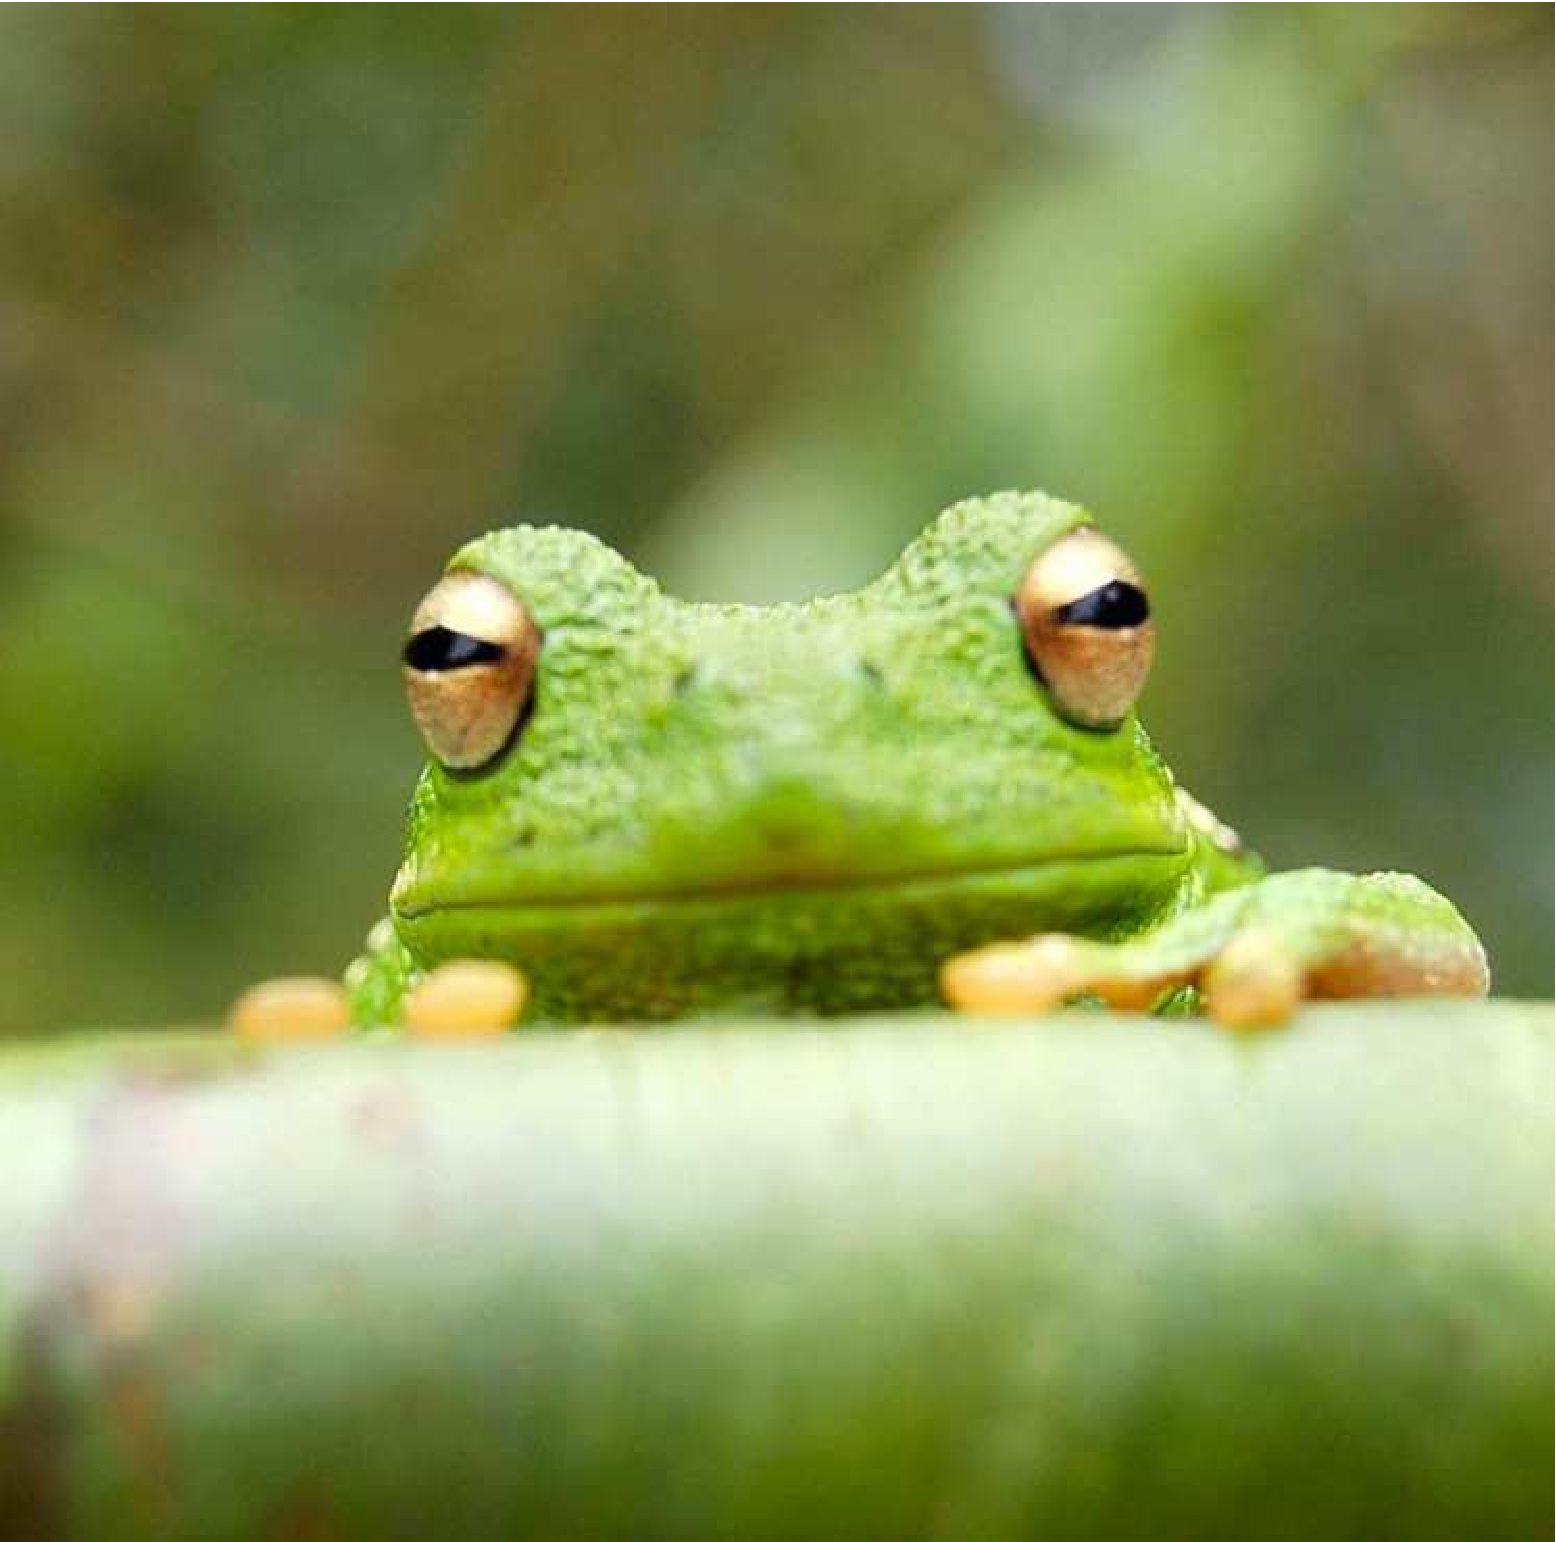
\includegraphics[width=.8\linewidth]{frog.pdf}
% \caption{Placeholder image of a frog with a long example legend to show justification setting.}
% \label{fig:frog1}
% \end{figure}


% \begin{figure*}[t!]
% \centering
% 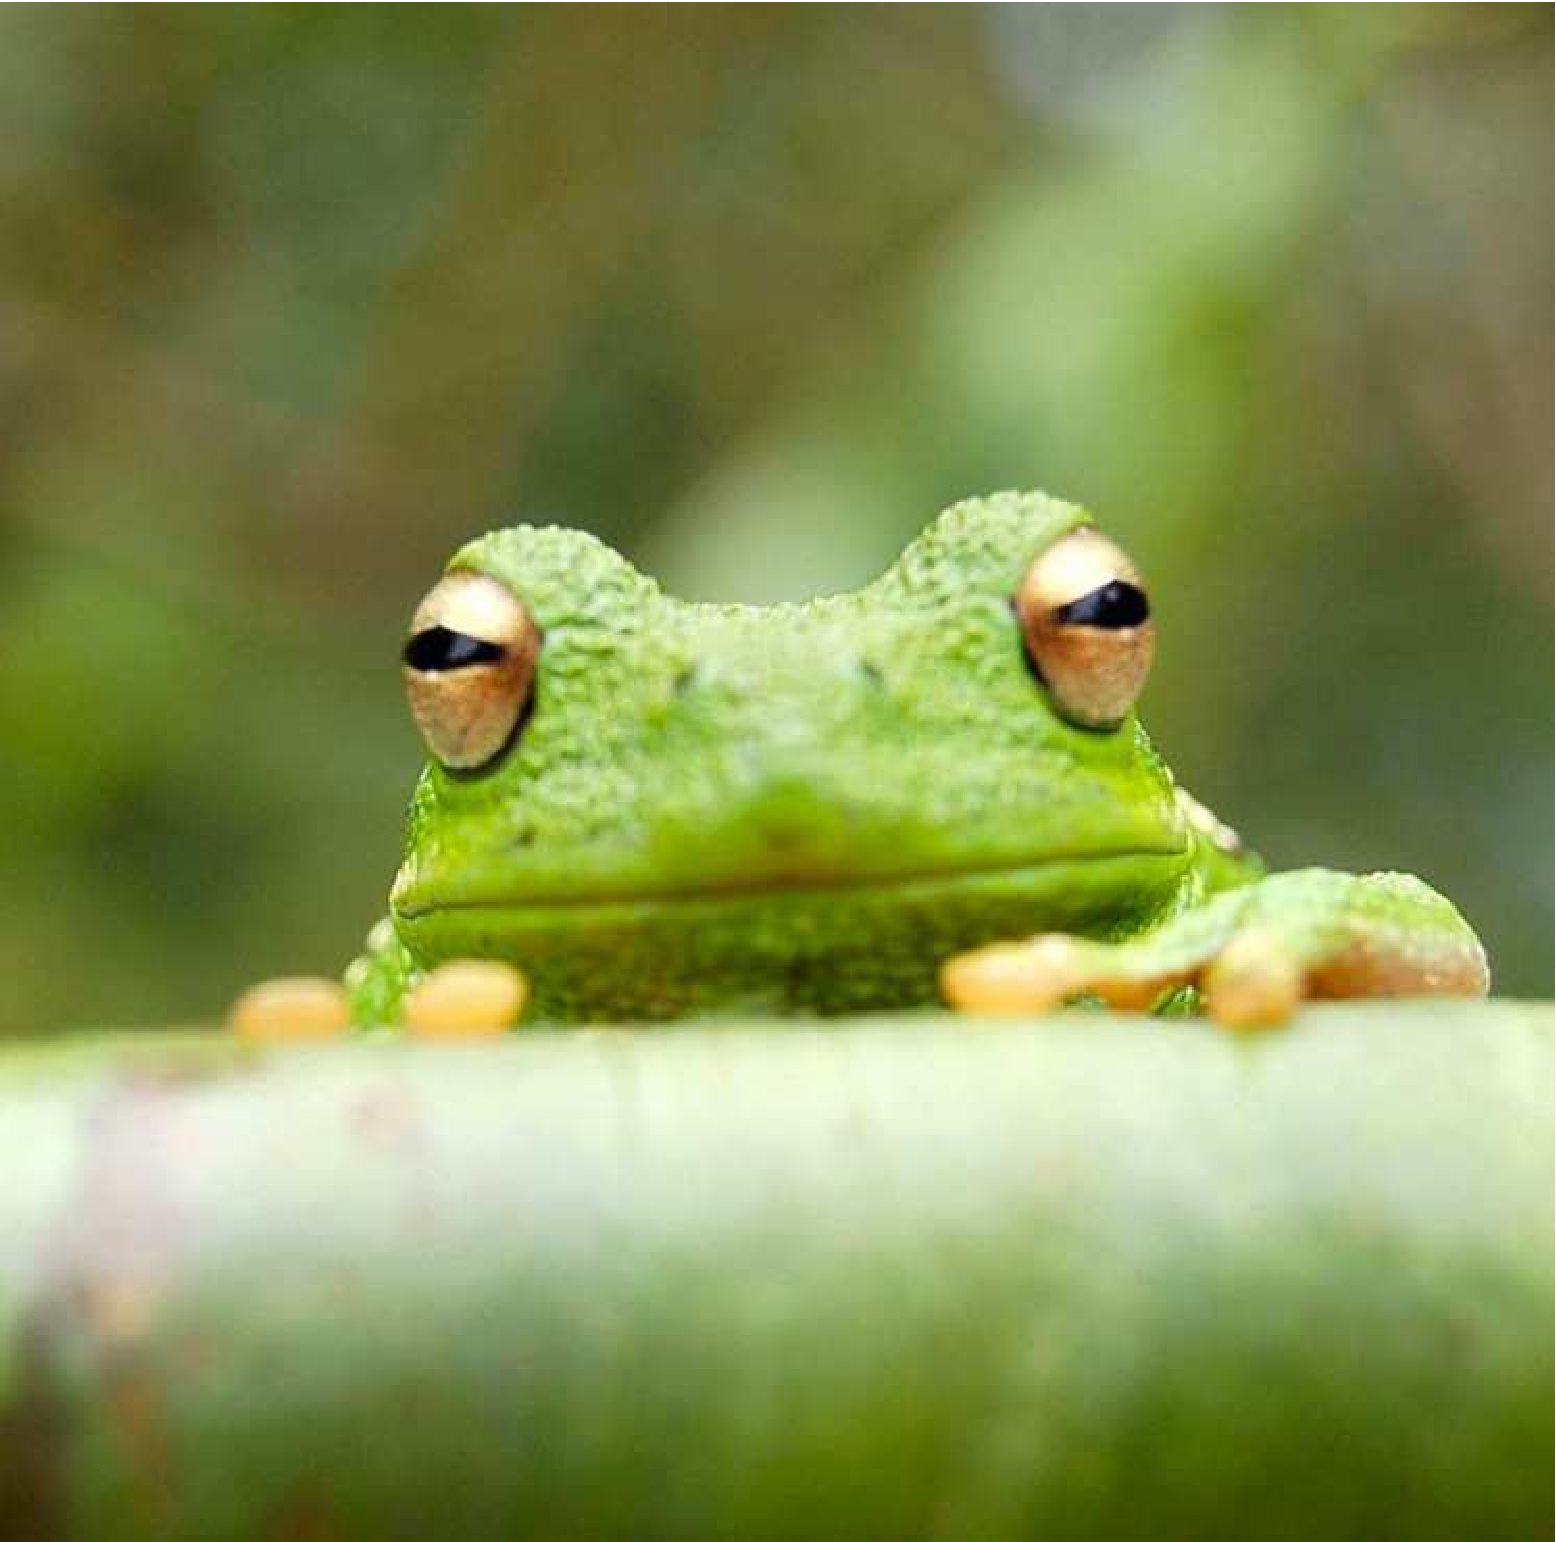
\includegraphics[scale=0.6]{frog}
% \caption{Placeholder image of a frog with a long example legend to show justification setting.}
% \label{fig:frog2}
% \end{figure*}


% \begin{table}[t!]
% \centering
% \caption{Comparison of the fitted potential energy surfaces and ab initio benchmark electronic energy calculations}
% \begin{tabular}{lrrr}
% Species & CBS & CV & G3 \\
% \midrule
% 1. Acetaldehyde & 0.0 & 0.0 & 0.0 \\
% 2. Vinyl alcohol & 9.1 & 9.6 & 13.5 \\
% 3. Hydroxyethylidene & 50.8 & 51.2 & 54.0\\
% \bottomrule
% \end{tabular}

% \addtabletext{nomenclature for the TSs refers to the numbered species in the table.}
% \end{table}


% \begin{table*}[t!]
% \centering
% \caption{Impact on Emission Behaviors by Socioeconomic Status}
% \begin{tabular*}{\textwidth}{@{\extracolsep{\fill}}lccccc@{}}
% & (1) & (2) & (3) & (4) & (5) \\
% \midrule
%  & \multicolumn{2}{c}{City-level} & Firm-level & \multicolumn{2}{c}{City-level} \\
% Dep. Var.: & \multicolumn{2}{c}{COD Emission (1,000 tons)} & COD Emission (ton) & Firm Entry & Firm Exit \\
% \multicolumn{6}{c}{Panel A: Population Share without College Education} \\
% Share of Below College $\times$ Post$_{05}$ & 0.165*** & 0.292** & 0.358*** & 0.623** & 0.280 \\
%  & (0.026) & (0.119) & (0.106) & (0.266) & (0.487) \\
% Share of Below College & -0.208 & & & & \\
%  & (0.141) & & & & \\
% Post$_{05}$ & -16.426*** & & & & \\
%  & (2.873) & & & & \\
% \multicolumn{6}{c}{Panel B: Population Share without High School Education} \\
% Share of Below HS $\times$ Post$_{05}$ & 0.099*** & 0.218** & 0.232** & 0.453** & 0.089 \\
%  & (0.005) & (0.090) & (0.079) & (0.195) & (0.333) \\
% Share of Below HS & -0.213* & & & & \\
%  & (0.100) & & & & \\
% Post$_{05}$ & -9.465*** & & & & \\
%  & (0.564) & & & & \\
% \bottomrule
% \end{tabular*}

% \addtabletext{*** P $<$ 0.01, ** P $<$ 0.05, * P $<$ 0.1}
% \end{table*}

% \subsection*{Digital Figures}

% EPS and high-resolution PDF are preferred formats for figures that will be used in the main manuscript. Authors may submit PRC or U3D files for 3D images; these must be accompanied by 2D representations in TIFF, EPS, or high-resolution PDF format. Color images must be in RGB (red, green, blue) mode. Include the font files for any text.

% Images must be provided at final size, preferably 1 column width (8.7cm). Figures wider than 1 column should be sized to 11.4cm or 17.8cm wide. Numbers, letters, and symbols should be no smaller than 6 points (2mm) and no larger than 12 points (6mm) after reduction and must be consistent.

% Figures and tables should be labelled and referenced in the standard way using the \verb|\label{}| and \verb|\ref{}| commands.

% Figure \ref{fig:frog1} shows an example of how to insert a column-wide figure. To insert a figure wider than one column, please use the \verb|\begin{figure*}...\end{figure*}| environment. Figures wider than one column should be sized to 11.4 cm or 17.8 cm wide. Use \verb|\begin{SCfigure*}...\end{SCfigure*}| for a wide figure with side legends.

% \begin{SCfigure*}[\sidecaptionrelwidth][t!]
% \centering
% 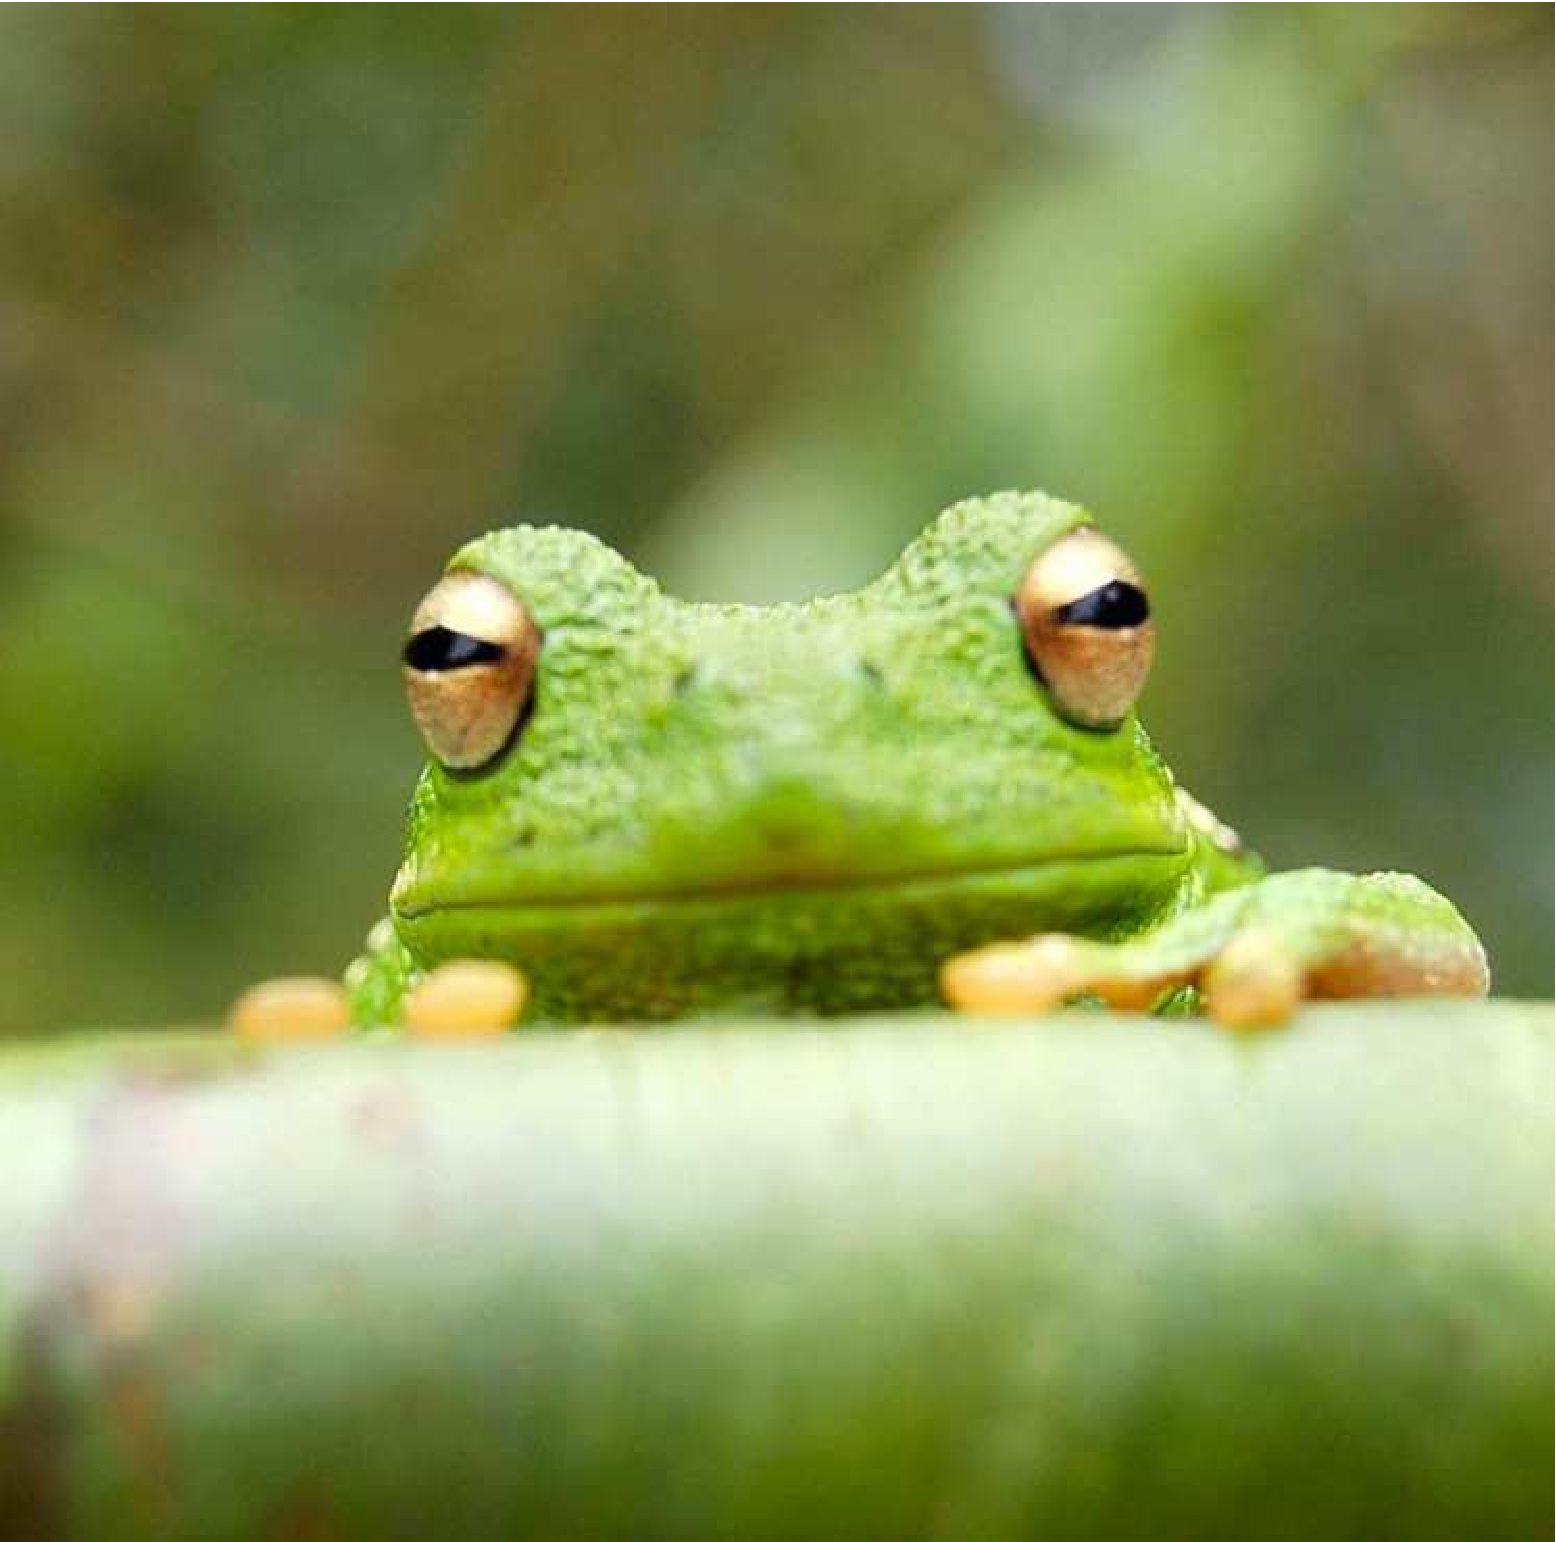
\includegraphics[width=11.4cm,height=11.4cm]{frog.pdf}
% \caption{This legend would be placed at the side of the figure, rather than below it.}\label{fig:side}
% \end{SCfigure*}


% \subsection*{Tables}
% Tables should be included in the main manuscript file and should not be uploaded separately.


% \subsection*{Footnotes}

% Footnotes are ordered by symbols such as *, \textdagger, \textdaggerdbl, etc. The article should contain only 13 footnotes\footnote{Footnote Example 1}\footnote{Footnote Example 2}.


% \subsection*{Single column equations}

% Authors may use 1- or 2-column equations in their article, according to their preference.

% \begin{align*}
% (x+y)^3&=(x+y)(x+y)^2\\
%        &=(x+y)(x^2+2xy+y^2) \numberthis \label{eqn:example1} \\
%        &=x^3+3x^2y+3xy^3+x^3.
% \end{align*}

% To allow an equation to span both columns, use the \verb|\begin{figure*}...\end{figure*}| environment mentioned above for figures.

% Note that the use of the \verb|widetext| environment for equations is not recommended, and should not be used.

% \begin{figure*}[bt!]
% \begin{align*}
% (x+y)^3&=(x+y)(x+y)^2\\
%        &=(x+y)(x^2+2xy+y^2) \numberthis \label{eqn:example2} \\
%        &=x^3+3x^2y+3xy^3+x^3.
% \end{align*}
% \end{figure*}



% \subsection*{Supporting Information Appendix (SI)}

% Authors should submit SI as a single separate SI Appendix PDF file, combining all text, figures, tables, movie legends, and SI references. SI will be published as provided by the authors; it will not be edited or composed. Additional details can be found in the \href{https://www.pnas.org/author-center/submitting-your-manuscript#supporting-information}{PNAS Author Center}. The PNAS Overleaf SI template can be found \href{https://www.overleaf.com/latex/templates/pnas-template-for-supplementary-information/wqfsfqwyjtsd}{here}. Refer to the SI Appendix in the manuscript at an appropriate point in the text. Number supporting figures and tables starting with S1, S2, etc.

% Authors who place detailed materials and methods in an SI Appendix must provide sufficient detail in the main text methods to enable a reader to follow the logic of the procedures and results and also must reference the SI methods. If a paper is fundamentally a study of a new method or technique, then the methods must be described completely in the main text.

% Supporting information (SI) for PNAS Brief Reports is limited to extended methods, essential supporting datasets, software, and video/audio files; supporting text, tables or figures are not permitted.

% \subsubsection*{SI Datasets}

% Supply .xlsx, .csv, .txt, .rtf, GZ or .pdf files. This file type will be published in raw format and will not be edited or composed.


% \paragraph*{SI Movies}

% Supply Audio Video Interleave (avi), Quicktime (mov), Windows Media (wmv), animated GIF (gif), or MPEG-4 Part 14 (mp4) files. Movie legends should be included in the SI Appendix file. All movies should be submitted at the desired reproduction size and length. Movies should be no more than 10MB in size.



% \matmethods{Please describe your materials and methods here. This can be more than one paragraph, and may contain subsections and equations as required. If your research involved human or animal participants, please identify the institutional review board and/or licensing committee that approved the experiments. Please also include a brief description of your informed consent procedure if your experiments involved human participants.


% \subsection*{Subsection for Method}
% Example text for subsection.
% }

% \showmatmethods{} % Display the Materials and Methods section

% \dataavail{To allow others to replicate and build on work published in PNAS, authors must make materials, data, and associated protocols, including code and scripts, available to readers in a public repository upon publication. Restrictions on full or partial access to these materials and requests for legal, ethical, and logistical (e.g., size) exceptions must be noted at submission. If requested, these materials must be made available to editors and reviewers during submission for the purpose of evaluating the manuscript. A statement detailing sharing plans will be included in the published article as provided within the submission form. Research datasets, whether original or previously published, must be cited in the references as a condition for publication. Please refer to our full \href{https://www.pnas.org/author-center/editorial-and-journal-policies\#materials-and-data-availability}{policy}.}

% \acknow{Please include your acknowledgments here, set in a single paragraph. Please do not include any acknowledgments in the Supporting Information, or anywhere else in the manuscript.}

% \showacknow{} % Display the acknowledgments section




% \bibsplit[3]
% %Use \bibsplit to split the references from the body of the text. Value "[3]" represents the number of reference in the left column (Note: Please avoid single column figures & tables on this page.)

% Bibliography
\bibliography{pnas-sample}

\end{document}
